%% Document class
\documentclass[12pt,preprint]{aastex}
%\documentclass[preprint2]{aastex}

%general packages
\usepackage{amsmath}	%for \text{} in math mode
\usepackage{mathrsfs } %for likelihood L
%\usepackage{lscape} % landscape environment

%%Figure packages
\usepackage{grffile}	%for dots in filenames

%% Custom macros
\newcommand{\vect}[1]{\boldsymbol{#1}} % Uncomment for BOLD vectors.
%\newcommand{\vect}[1]{\vec{#1}} % Uncomment for ARROW vectors.
\newcommand*\diff{\mathop{}\!\mathrm{d}}
\newcommand*\Diff[1]{\mathop{}\!\mathrm{d^#1}}
\newcommand{\pdf}{\ensuremath{pdf}}
\newcommand{\pmodel}{\ensuremath{p_M}}
\newcommand{\MAP}{{\sl MAP~}}
\newcommand{\MAPs}{{\sl MAP}s~}
\newcommand{\RM}{{\sl RoadMapping~}}
 
%% Abbreviations
\shorttitle{Action-based Dynamical Models for the Milky Way}
\shortauthors{Trick et al.}

\begin{document}

%% Title
\title{The {\sc RoadMapping} Code:\\How to deal with "Real World" Issues\\in Action-based Dynamical Modelling the Milky Way\\}

%% Authors    
\author{W. Trick\altaffilmark{1,2},  J. Bovy\altaffilmark{3,4}, and H.-W. Rix\altaffilmark{1}}
\email{trick@mpia.de}

%% Affiliations
\altaffiltext{1}{Max-Planck-Institut f\"ur Astronomie, K\"onigstuhl 17, D-69117 Heidelberg, Germany}
\altaffiltext{2}{Correspondence should be addressed to trick@mpia.de.}
\altaffiltext{3}{Institute for Advanced Study, Einstein Drive, Princeton, NJ 08540, USA}
\altaffiltext{4}{Hubble fellow}


%%-----------------------------------------------------------------------------------------------------------------------------------------------------------------------------
% Abstract
\begin{abstract}
Starting point for abstract: my old poster abstract. [TO DO] We aim to recover the Milky Way's gravitational potential using action-based dynamical modeling (cf. Bovy \& Rix 2013, Binney \& McMillan 2011, Binney 2012). This technique works by modeling the observed positions and velocities of disk stars with an equilibrium, three-integral quasi-isothermal distribution function. In preparation for the application to stellar phase-space data from Gaia, we create and analyze a large suite of mock data sets and we develop qualitative "rules of thumb" for which characteristics and limitations of data, model and code affect constraints on the potential most. We investigate sample size and measurement errors of the data set, size and shape of the observed volume, numerical accuracy of the code and action calculation, and deviations of the data from the assumed family of axisymmetric model potentials and distribution functions. This will answer the question: What kind of data gives the best and most reliable constraints on the Galaxy's potential?
\end{abstract}}
%-----------------------------------------------------------------------------------------------------------------------------------------------------------------------------

%% Keywords
\keywords{Galaxy: disk --- Galaxy: fundamental parameters --- Galaxy: kinematics and dynamics --- Galaxy: structure}

%table of contents (remove later)
\tableofcontents

%-----------------------------------------------------------------------------------------------------------------------------------------------------------------------------
%Introduction
\section{Introduction} \label{sec:intro}

%Everything in a nutshell
Stellar dynamical modelling is the fundamental tool to infer the gravitational potential of the Milky Way from the positions and motions of its stars \citep{rix13,bin11b} [TO DO]. The observational information on the phase-space coordinates of stars are currently growing at a rapid pace, and will be taken to a whole new level by the upcoming Gaia data. Yet, rigorous and practical modelling tools that turn this information into constraints both on the gravitational potential and on the distribution function (DF) of stellar orbits, are scarce \citep{rix13} [TO DO: more references] [TO DO: References that explain that the modelling is scarce, or previous modelling approaches???]

[TO DO: Modelling tools for the MW: 
a) Made-to-measure: 
\citet{lor07}(based on \citet{sye96} , best application to to bulge \citet{bis04}, 
\citet{hun14} also have a tool for Gaia at hand, 
b) Streams: 
\citet{joh99} 
c) Action-based distribution function modelling
\citet{san15}
\citet{pif14}
d) torus modelling
e) Jeans modelling
\citet{bue15}
\citet{loe12}]



%Papers In which I am looking for references:
%http://arxiv.org/pdf/1104.2839v1.pdf
%http://arxiv.org/pdf/1301.3168v1.pdf, Rix & Bovy 2013, continue on page 13
%http://arxiv.org/pdf/1108.1749v2.pdf

%Why potential + DF are important
Accurately determining the Galactic gravitational potential is fundamental for understanding its dark matter and baryonic structure [REF]. Accurately determining the stellar-population dependent orbit distribution function is a fundamental contraint on the Galaxy's formation history. \\

%In more detail: Why potential is important
Open questions about the MW's potential and structure, on which future modelling attempts will hopefully give more definite answers are: What is the local dark matter density \citep{zha13,bt12}? Is the Milky Way's dark matter halo flattened ([REF])? Is the MW disk maximal \citep{sac97} and, to be able to disentangle halo and disk contribution \citep{deh98}, what is the disk's overall mass scale length \citep{bov13}?  \\

%In more detail: Why DF is important
Open questions about the star's distribution within the MW, which dynamical modelling can help to constrain, are: How are stellar kinematics and their chemical abundances are related (\cite{san15},[REF])? In particular, does the disk have a thin/thick disk dichotomy (\cite{gil83}) or is it a continuum of many exponential disks (\cite{bov12d})? How does radial migration affect the orbit distribution \citep{sel02,ros08a,ros08b,sch08,min11} [TO DO: These are References from Rix \& Bovy 2013 - should I use all of them?]?\\
To address these questions, observed stellar positions and motions need to be turned into full orbits - which stresses again the importance of having a reliable model for the MW's gravitational potential. \\

%The era of big Galactic surveys (the big motivation behind our work)
In the era of big Galactic surveys all of this could soon be within our reach. Not only will there be full 6D stellar phase-space coordinates for a thousand million of stars measured by Gaia to unprecedented precision by the end of 2016. But already with existing surveys (e.g., SEGUE (Beers et al. 2006), RAVE (Steinmetz et al. 2006), LAMOST (Newberg et al. 2012), APOGEE (Majewski 2012), Gaia-ESO (Gilmore et al. 2012), GALAH (Freeman 2012) [TO DO: I just copied this from Melissas Cannon paper. Should I reference all of them??? Not in reference list yet.]) and sophisticated machine-learning tools (e.g. \emph{The Cannon} by \cite{nes15}) to combine them, we will soon have huge data sets at our disposal.

%This works actual objective
In this work we present a rigorous, robust and reliable dynamical modelling machinery, strongly building on previous work by \citet{bin11,bin12,bov13,bov15} and explicitly developed to exploit and deal with these large data sets in the future.

%Action-based DF modelling in general
There is a variety of practical approaches to dynamical modelling of discrete collisionless tracers (such as the stars in the Milky Way) [REF]. Most of them -- explicitly or implicitly -- describe the stellar distribution through a distribution function.  Actions are good ways to describe orbits, because they are canonical variables with their corresponding angles, have immediate physical meaning, and obey adiabatic invariance [Binney 2011abcdefg???]. \\

%The roots of our approach
Recently, \cite{bin12b} and \cite{bov13} [TO DO: are these the correct references???] proposed to combine parametrized axisymmetric potentials with DF's that are simple analytic functions of the three orbital actions to model discrete data. \cite{bin10} and \cite{bin11} had proposed a set of simple action-based (quasi-isothermal) distribution functions (qDF). \cite{Tin13} and \cite{bov13} showed that these qDF's may be good descriptions of the Galactic disk, when one only considers so-called mono-abundance populations (\MAP), i.e. sub-sets of stars with similar [Fe/H] and [$\alpha$/Fe] (\cite{bov12b}, \cite{bov12c}, \cite{bov12d}). \\

%The first version of the code + first results
\cite{bov13} implemented a modelling approach that put action-based DF modelling of the Galactic disk in an axisymmetric potential in practice. Given an assumed potential and an assumed DF, they directly calculated the likelihood of the observed ($\vec{x},\vec{v}$) for each sub-set of \MAP among SEGUE Gdwarf \citep{yan09}. This modelling also accounted for the complex, but known selection function of the kinematic tracers.  For each \MAP, the modelling resulted in a constraint of its DF, and an independent constraint on the gravitational potential, which members of all \MAPs feel the same way. \\
Taken as an ensemble, the individual \MAP models constrained the disk surface mass density over a wide range of radii ($\sim 4-9$ kpc), and proved a powerful constraint on the disk mass scale length ($\sim 2$ kpc) and on the disk to dark matter ratio at the Solar radius [TO DO: quote number???]. \\

%Drawbacks of the first code version in the era of large surveys
Yet, these recent models still leave us poorly prepared with the wealth and quality of the existing and upcoming data sets. This is because \cite{bov13} made a number of quite severe and idealizing assumptions about the potential, the DF and the knowledge of observational effects (such as the selection function). All these idealizations are likely to translate into systematic error on the inferred potential or DF, well above the formal error bars of the upcoming data sets. \\

%Focus of this work: Not just follow-up of BR13, but presentation and investigation of much improved machinery
In this work we present \RM ("\textsc{R}ecovery of the \textsc{O}rbit \textsc{A}ction \textsc{D}istribution of \textsc{M}ono-\textsc{A}bundance \textsc{P}opulations and \textsc{P}otential \textsc{IN}ference for our \textsc{G}alaxy") - an improved and refined version of the original modelling machinery by \cite{bov13}, making extensive use of the \emph{galpy} python package (\cite{bov15}). \RM relaxes some of the restraining assumptions \cite{bov13} had to made, is more flexible and more adept in dealing with large data sets. In this paper we set out to explore the robustness of \RM against the breakdowns of some of the most important assumptions of DF-based dynamical modelling. What is it about the data, the model and the machinery itself, that limits our recovery of the true gravitational potential? \\

%Large Data + Machinery
In the light of Gaia we explicitely analyze how well the modelling machinery behaves in the limit of large data. For a huge number of stars three statistical aspects become important, that are  hidden behind Poisson noise for smaller data sets: (i) We have to make sure that our modelling is an un-biased and asymptotically normal estimator (\S\ref{sec:largedata}). (ii) Numerical inaccuracies in the actual modelling machinery start to matter and need to be avoided (\S\ref{sec:numaccuracynormalisation}). (iii) Parameter estimates become so precise, that we start to be able to distinguish between similar models. We therefore want more flexibility and more free fit parameters in the potential and DF model. The modelling machinery itself needs to be flexible and fast in effectively finding the best fit parameters for a large set of parameters. The improvements made to the machinery used in \cite{bov13} are presented in \S\ref{sec:fitting}. \\

%Data 
Different characteristics of the data might influence the success of the parameter recovery. (i) In an era where we can choose data from different MW surveys, it might be worth to explore if different regions within the MW (i.e. differently shaped or positioned survey volumes) are especially diagnostic to recover the potential (\S\ref{sec:result_obsvolume}). (ii) What happens if our knowledge about the selection function, specifically the completeness of the data set within the survey volume, is not perfect (\S\ref{sec:results_incompR})? (iii) How to account for measurement errors in the modelling (\S\ref{sec:results_errors})? \\

%Model
One of the strongest assumptions is to restrict the dynamical modelling to a certain family of parametrized models. We investigate how well we can we hope to recover the true potential, when our potential and DF models deviate from the true potential and DF. For the DF we specifically investigate two of our assumptions in \S\ref{sec:results_mixedDFs}: First, what would happen if the stars within \MAPs do intrinsically not follow a single qDF as assumed by \cite{tin13,bov13}. Second, and assuming \MAPs do indeed follow the qDF, what would be the effect of pollution of \MAPs through stars from neighbouring \MAPs in the ([Fe/H],[$\alpha$/Fe]) plane due to too big abundance errors or bin sizes.\\
And last but not least we test in \S\ref{sec:potential} how well the modelling works, if our assumed potential family deviaties from the true potential. \\

For all of these aspects we show some plausible and illustrative examples on the basis of investigating mock data. The mock data is generated from galaxy models presented in \S\ref{sec:potentials}-\ref{sec:selectionfunction} following the procedure in \S\ref{sec:mockdata}, analysed according to the description of the machinery in \S\ref{sec:likelihood}-\ref{sec:fitting} and the results are presented in \S\ref{sec:results} and discussed in \S\ref{sec:discussionsummary}.\\

The strongest assumption that goes into this kind of dynamical modelling might be the idealization of the Galaxy to be axi-symmetric and being in steady state. We do not investigate this within the scope of this paper but strongly suggest a systematic investigation of this for future work.

}
%-----------------------------------------------------------------------------------------------------------------------------------------------------------------------------

%-----------------------------------------------------------------------------------------------------------------------------------------------------------------------------
%Dynamical Modelling
\subsection{Actions and Potential Models}  \label{sec:potentials}

\paragraph{Actions.} Orbits in axisymmetric potentials are best described and fully specified by the three actions $J_R, J_z$ and $J_\phi=L_z$. They are integrals of motion and generally defined as
\begin{equation}
J_i = \frac{1}{2\pi} \int_\text{orbit} p_i(t) \diff x_i(t) \label{eq:action_general}
\end{equation}
and depend on the potential via the connection between position $x_i$ and momentum $p_i$ along the orbit. Actions have a clear physical meaning: They quantify the amount of oscillation in each coordinate direction of the full orbit [REF]. The position of a star along the orbit is denoted by a set of angles, which form together with the angles a set of canonical conjugate phase-space coordinates \citep{bin08}. Even though actions are the optimal choice as orbit labels and arguments for stellar distribution functions, their computation is very expensive.

\paragraph{Action calculation.} The action calculation depends on the choice of potential in which the star moves: The spherical isochrone \citep{bin08} is the only potential for which Eq. (\ref{eq:action_general}) takes an analytic form. For axisymmetric St\"{a}ckel potentials actions can be calculated exactly by the (numerical) evaluation of a single integral. In all other potentials numerically calculated actions will always be approximations, unless Eq. (\ref{eq:action_general}) is integrated up to infinity.  A computational fast way to get actions for arbitrary axisymmetric potentials is the "St\"{a}ckel fudge" by \citet{bin12}, which locally approximates the potential by a St\"{a}ckel potential. To speed up the calculation even more, an interpolation grid can be build out of these St\"{a}ckel fudge actions, as described in \citet{bov15}. 

\paragraph{Potential models.} In our modelling we assume a family of parametrized potentials with a fixed number of free parameters. We use different kinds of potentials: Besides the Milky Way like potential from \citet{bov13} ("MW13-Pot" ) with bulge, disk and halo, we also extensively use the spherical isochrone potential ("Iso-Pot") in our test suites to make use of the analytic (and therefore exact and fast) way  to calculate actions. In addition we use the 2-component Kuzmin-Kutuzov St\"{a}ckel potential by \citet{bat94} ("KKS-Pot"), which displays a disk and halo structure and also provides exact actions. Table \ref{tbl:referencepotentials} summarizes all reference potentials together used in this work with their free parameters $p_\Phi$. The density distribution of these potentials is illustrated in Fig. \ref{fig:ref_pots}.

%======================================================================================

\begin{deluxetable}{llllll}
\tabletypesize{\scriptsize}
\rotate
\tablecaption{Gravitational potentials of the reference galaxies used troughout this work and the respective ways to calculate actions in these potentials. All four potentials are axisymmetric. The potential parameters are fixed for the mock data creation. In the subsequent analyses we aim to recover these potential parameters again. The parameters of "MW13-Pot" and "KKS-Pot" were found as best fits to the "MW14-Pot". \label{tbl:referencepotentials}}
\tablewidth{0pt}
\tablehead{
\colhead{name} & \colhead{potential type} & \multicolumn{2}{c}{potential parameters $p_\Phi$} & \colhead{action calculation} & \colhead{reference for potential type}}
\startdata
"Iso-Pot" & isochrone potential   & circular velocity at the sun             & $v_\text{circ}$ = $230$ km s$^{-1}$           & \textbf{\emph{analytical and exact}} $J_r, J_\vartheta, L_z$;     & \citet{bin08} \\
          &					      & isochrone scale length                   & $b$ = $0.9$ kpc                               & use $J_r \rightarrow J_R, J_\vartheta \rightarrow J_z $  &               \\
          &                       &                                          &                                               & in eq. (???)                                             &               \\
\tableline
"KKS-Pot" & 2-component                  & circular velocity at the sun             & $v_\text{circ}$ = $230$ km s$^{-1}$           & \textbf{\emph{exact}} $J_R, J_z, L_z$       & \citet{bat94} \\
          & Kuzmin-Kutuzov-              & focal distance of coordinate system\tablenotemark{a}       & $\Delta = 0.3$              & using "St\"{a}ckel Fudge"                   &               \\                                                                
          & St\"{a}ckel potential        & axis ratio of the coordinate surfaces\tablenotemark{a} ... &                             & \citep{bin12}                               &               \\
          & \hspace{0.3cm} (disk + halo) & \hspace{0.3cm} ...of the disk component   & $\left(\frac{a}{c}\right)_\text{Disk}$ = 20  & and interpolation                           &               \\
          &                              & \hspace{0.3cm} ...of the halo component   & $\left(\frac{a}{c}\right)_\text{Halo}$ = 1.07& on action grid                              &               \\
          & (analytic potential)         & relative contribution of the disk mass    &                                              & \citep{bov15}                               &               \\
          &                              & \hspace{0.3cm} to the total mass          & $k = 0.28$                                   &                                             &               \\  
\tableline
"MW13-Pot" & MW-like potential with        & circular velocity at the sun             & $v_\text{circ}$ = $230$ km s$^{-1}$           & \textbf{\emph{approximate}} $J_R, J_z, L_z$ & \citet{bov13} \\          
           & Hernquist bulge,              & stellar disk scale length                & $R_d = 3$ kpc                                 & using "St\"{a}ckel Fudge"          &               \\
           & 2 exponential disks           & stellar disk scale height                & $z_h = 0.4$ kpc                               & \citep{bin12}                      &               \\
           & \hspace{0.3cm} (stars + gas), & relative halo contribution to $v_\text{circ}^2(R_\odot)$ & $f_h = 0.5$                   & and interpolation                  &               \\
           & spherical power-law halo      & "flatness" of rotation curve & $\frac{\diff \ln(v_\text{circ}(R_\odot))}{ \diff \ln(R)}$ = 0  & on action grid                &               \\
           & (interpolated potential)      &                                          &                                               & \citep{bov15}                      &               \\
\tableline
"MW14-Pot" & MW-like potential with        &  -                                       & -                                             & \textbf{\emph{approximate}} $J_R, J_z, L_z$ & \citet{bov15} \\
           & cutoff power-law bulge,       &                                          &                                               & (see "MW13-Pot")                   &               \\
           & Miyamoto-Nagai stellar disk,  &                                          &                                               &                                    &               \\
           & NFW halo                      &                                          &                                               &                                    &               \\
\enddata
\tablenotetext{a}{The coordinate system of each of the two St\"{a}ckel-potential components is $\frac{R^2}{\tau_{i,p}+\alpha_p} + \frac{z^2}{\tau_{i,p}+\gamma_p}=1$ with $p \in \{\text{Disk},\text{/Halo}\}$ and $\tau_{i,p} \in \{\lambda_p,\nu_p\}$. Both components have the same focal distance $\Delta = \sqrt{\gamma_p-\alpha_p}$, to make sure that the superposition of the two components itself is still a St\"{a}ckel potential. The axis ratio of the coordinate surfaces $\left(\frac{a}{c}\right)_p := \sqrt{\frac{\alpha_p}{\gamma_p}}$ describes the flattness of the corresponding St\"{a}ckel component.}
\end{deluxetable}

%=============================================

%FIGURE: reference potentials

\begin{figure}
\plotone{figs/reference_potentials.eps}
\caption{Density distribution of the four reference galaxy potentials in table \ref{tbl:referencepotentials}, for illustration purposes. These potentials are used throughout this work for mock data creation and potential recovery. [TO DO: Halo sichtbarer machen, evtl. mit isodensity contours]}
\label{fig:ref_pots}
\end{figure}

%=============================================

\subsection{Distribution Function} \label{sec:qDF}

\paragraph{Distribution Function.} Motivated by the findings of Bovy et al. 2012??? and \citet{tin13} about the simple phase-space structure of \MAPs, and following \citet{bov13} and their successful application, we also assume that each \MAP follows a single qDF of the form given by \citet{bin11}.  This qDF  is a function of the actions $\vect{J}=(J_R,J_z,L_z)$ and has the form
\begin{eqnarray}
\text{qDF}(\vect{J} \mid p_\text{DF}) &=& f_{\sigma_R}\left(J_R,L_z \mid p_\text{DF}\right) \times f_{\sigma_z}\left(J_z,L_z \mid p_\text{DF}\right)\label{eq:df_general}\\
\text{with } f_{\sigma_R}\left(J_R,L_z \mid p_\text{DF}\right) &=& n \times \frac{\Omega}{\pi\sigma_R^2(R_g) \kappa}\left[1+\tanh\left(L_z/L_0\right) \right]\exp\left(-\frac{\kappa J_R}{\sigma_R^2(R_g)} \right) \\
f_{\sigma_z}\left(J_z,L_z \mid p_\text{DF} \right) &=& \frac{\nu}{2 \pi \sigma_z^2(R_g)} \exp\left( -\frac{\nu J_z}{\sigma_z^2(R_g)} \right) \\
\end{eqnarray}
Here $R_g \equiv R_g(L_z)$ and $\Omega\equiv \Omega(L_z)$ are the (guidig-center) radius and the circular frequency of the circular orbit with angular momentum $L_z$ in a given potential. $\kappa\equiv \kappa(L_z)$ and $\nu\equiv \nu(L_z)$ are the radial/epicycle ($\kappa$) and vertical ($\nu$) frequencies with which the star would oscillate around the circular orbit in $R$- and $z$-direction when slightly perturbed \citep{bin08}. The term $\left[1+\tanh\left(L_z/L_0\right) \right]$ suppresses counter-rotation for orbits in the disk with $L \gg L_0$ which we set to a random small value ($L_0 = 10 \times R_\odot/8 \times v_\text{circ}(R_\odot)/220$).
\\For this qDF to be able to incorporate the findings by Bovy et al. 2012??? about the phase-space structure of \MAPs summarized in \S\ref{sec:intro}, we set the functions $n$,  $\sigma_R$ and $\sigma_z$, which indirectly set the stellar number density and radial and vertical velocity dispersion profiles,
\begin{eqnarray}
n(R_g \mid p_\text{DF}) &\propto& \exp\left(-\frac{R_g}{h_R} \right)\\
\sigma_R(R_g \mid p_\text{DF}) &=& \sigma_{R,0} \times \exp\left(- \frac{R_g-R_\odot}{h_{\sigma_R}} \right)\label{eq:sigmaRRg}\\
\sigma_z(R_g \mid p_\text{DF}) &=& \sigma_{z,0} \times \exp\left(- \frac{R_g-R_\odot}{h_{\sigma_z}} \right)\label{eq:sigmazRg}.
\end{eqnarray}
The qDF for each \MAP has therefore a set of five free parameters $p_\text{DF}$: the density scale length of the tracers $h_R$, the radial and vertical velocity dispersion at the solar position $R_\odot$, $\sigma_R,0$ and $\sigma_z,0$, and the scale lengths $h_{\sigma_R}$ and $h_{\sigma_z}$, that describe the radial decrease of the velocity dispersion. The \MAPs we use for illustration through out this work are summarized in Table \ref{tbl:referenceMAPs}.

\paragraph{Tracer Density.} One crucial point in our dynamical modelling technique (\S ???), as well as in creating mock data (\S\ref{sec:mockdata}), is to calculate the (axisymmetric) spatial tracer density $\rho_\text{DF}(\vect{x} \mid p_{\Phi},p_\text{DF})$ for a given qDF and potential . We do this by integrating the qDF at a given $(R,z)$ over all three velocity components, using a $N_\text{velocity}$-th order Gauss-Legendre quadrature for each integral:
\begin{eqnarray}
\rho_\text{DF}(R,|z| \mid p_{\Phi},p_\text{DF}) &=& \int_{-\infty}^{\infty} \text{qDF}(\vect{J}[R,z,\vect{v} \mid p_{\Phi}] \mid p_\text{DF}) \Diff3\vect{v}  \label{eq:tracerdensity_general}\\
&\approx& \int_{-N_\text{sigma} \sigma_R(R \mid p_\text{DF})}^{N_\text{sigma} \sigma_R(R \mid p_\text{DF})} \int_{-N_\text{sigma}\sigma_z(R \mid p_\text{DF})}^{N_\text{sigma} \sigma_z(R \mid p_\text{DF})} \int_{0}^{1.5 v_\text{circ}(R_\odot)}  \nonumber\\
& & \hspace{1cm} \text{qDF}(J[R,z,\vect{v} \mid p_{\Phi}] \mid p_\text{DF}) \diff v_T \diff v_z \diff v_R, \label{eq:tracerdensity}
\end{eqnarray}
where $\sigma_R(R \mid p_\text{DF})$ and $\sigma_z(R \mid p_\text{DF})$ are given by eq. (\ref{eq:sigmaRRg}) and (\ref{eq:sigmazRg}) and the integration ranges are motivated by Fig. \ref{fig:mockdatadistr}. For a given $p_\Phi$ and $p_\text{DF}$ we explicitly calculate the density on $N_\text{spatial} \times N_\text{spatial}$ regular grid points in the $(R,z)$ plane; in between grid points the density is evaluated with a bivariate spline interpolation. The grid is chosen to cover the extent of the observations for $z>0$. The total number of actions that need to be calculated to set up the density interpolation grid is $N_\text{spatial}^2 \cdot N_\text{velocity}^3$. Fig. ??? shows the importance of choosing $N_\text{spatial}$, $N_\text{velocity}$ and $N_\text{sigma}$ sufficiently large in order to get the density with an acceptable numerical accuracy. 

%======================================================================================

\begin{deluxetable}{lccccc}
\tabletypesize{\scriptsize}
%\rotate
\tablecaption{Reference distribution function parameters for the qDF in eq. (\ref{eq:df_general})-(\ref{eq:sigmazRg}). These qDFs describe the phase-space distribution of stellar \MAPs for which mock data is created and analysed throughout this work for testing purposes. The parameters of the "cooler" \& "colder"  ("hotter" \& "warmer") \MAPs were chosen such, that the they have the same $\sigma_R/\sigma_z$ ratio as the "hot" ("cool") \MAP. The "colder" and "warmer" \MAPs have a free parameter $X$ that governs how much colder/warmer they are then the reference "hot" and "cool" qDFs. Hotter populations have shorter tracer scale lengths \citep{bov12d} and the velocity dispersion scale lengths were fixed according to \citet{bov12c}. \label{tbl:referenceMAPs}}
\tablewidth{0pt}
\tablehead{
\colhead{name of \MAP} & \multicolumn{5}{c}{qDF parameters $p_\text{DF}$}\\
                       & \colhead{$h_R$ [kpc]} & \colhead{$\sigma_R$ [km s$^{-1}$]} & \colhead{$\sigma_z$ [km s$^{-1}$]} & \colhead{$h_{\sigma_R}$ [kpc]} & \colhead{$h_{\sigma_z}$ [kpc]}}
\startdata
"hot"    & 2   & 55 & 66 & 8 & 7\\
"cool"   & 3.5 & 42 & 32 & 8 & 7\\
\tableline
"cooler" & 2  +50\% & 55-50\% & 66-50\% & 8 & 7 \\
"hotter" & 3.5-50\% & 42+50\% & 32+50\% & 8 & 7\\
\tableline
"colder" & 2  +X\% & 55-X\% & 66-X\% & 8 & 7 \\
"warmer" & 3.5-X\% & 42+X\% & 32+X\% & 8 & 7\\
\enddata
\end{deluxetable}

%======================================================================================


\subsection{Selection Function}

\paragraph{Galactic Coordinate System.} Our modelling takes place in the Galactocentric rest-frame with cylindrical coordinates $\vect{x} \equiv (R,\phi,z)$ and corresponding velocity components $\vect{v} \equiv (v_R,v_\phi,v_z)$. If the stellar phase-space data is given in observed coordinates, position $\tilde{\vect{x}} \equiv(\alpha,\delta,m-M)$ in right ascension $\alpha$, declination $\delta$ and distance modulus $(m-M)$, and velocity $\tilde{\vect{v}} \equiv (\mu_\alpha,\mu_\delta,v_\text{los})$ as proper motions $\vect{\mu}=(\mu_\alpha,\mu_\delta)$ [TO DO: cos somwhere???] and line-of-sight velocity $v_\text{los}$, the data $(\tilde{\vect{x}},\tilde{\vect{v}})$ has to be converted first into the Galactocentric rest-frame coordinates $(\vect{x},\vect{v})$ using the sun's position and velocity. For simplicity we assume for the sun
\begin{eqnarray*}
(R_\odot,\phi_\odot,z_\odot) &=&(8 \text{ kpc}, 0^\circ, 0 \text{ kpc})\\
(v_{R,\odot},v_{T,\odot},v_{z,\odot}) &=& (0,230,0) \text{ km s}^{-1}.
\end{eqnarray*}

\paragraph{Selection Function.} A survey's selection function can be understood as a subvolume in the space of observables: e.g. position on the plane of the sky (limited by the pointing of the survey), distance from the sun (limited by the brightness of the stars and the sensitivity of the detector), colors and metallicity of the stars (limited by survey mode and targeting).
\\Within the framework of this paper, using only mock data for testing purposes, we ignore target cuts in colors and metallicity and simply use spatial selection functions, which we define as
\begin{eqnarray*}
\text{sf}(\vect{x}) \equiv \begin{cases}
\text{completeness}(\vect{x}) &\text{if $\vect{x}$ within observed volume}\\
0 & \text{outside}
\end{cases}
\end{eqnarray*}
It's value describes the probability to observe a star at $\vect{x}$. 
\\For the observed volume we use simple geometrical shapes: Either a sphere of radius $r_\text{max}$ with the sun at its center, or a "wedge", which we define as the angular segment of an cylindrical annuli, i.e. the volume with $R \in [R_\text{min},R_\text{max}],\phi \in [\phi_\text{min},\phi_\text{max}],z \in [z_\text{min},z_\text{max}]$ within the model galaxy.
\\The completeness is, in our framework, a function of position with $0 \leq \text{completeness}(\vect{x}) \leq 1$ everywhere inside the observed volume. It could be understood as a position-dependent detection probability. Unless explicitly stated otherwise, we use everywhere
$$\text{completeness}(\vect{x}) = 1.$$}
\subsection{Mock Data} \label{sec:mockdata}

One goal of this work is to test how the loss of information in the process of measuring stellar phase-space coordinates can affect the outcome of the modelling. To investigate this, we assume first that our measured stars do indeed come from our assumed families of potentials and distribution functions and draw mock data from a given true distribution. In further steps we can manipulate and modify these mock data sets to mimick observational effects.\\
The distribution function is given in terms of actions and angles. The transformation $(\vect{J}_i,\vect{\theta}_i) \longrightarrow (\vect{x}_i,\vect{v}_i)$ is however difficult to perform and computationally much more expensive than the transformation $(\vect{x}_i,\vect{v}_i) \longrightarrow (\vect{J}_i,\vect{\theta}_i)$. We propose a fast and simple two-step method for drawing mock data from an action distribution function, which also accounts effectively for a given survey selection function.


\paragraph{Preparation: Tracer density.} We first setup the interpolation grid for the tracer density $\rho(R,|z| \mid p_\Phi, p_\text{DF})$ generated by the given qDF and according to \S\ref{sec:qDF} and Eq. \ref{eq:tracerdensity}. For the creation of the mock data we use $N_\text{spatial} = 20$, $N_\text{velocity} = 40$ and $N_\text{sigma}=5$.

\paragraph{Step 1: Drawing positions from the selection function.} To get positions $\vect{x}_i$ for our mock data stars, we first sample random positions $(R_i,z_i,\phi_i)$ uniformly from the observed volume. Then we apply a rejection Monte Carlo method to these positions using the pre-calculated $\rho_\text{DF}(R,|z| \mid p_{\Phi},p_\text{DF})$. In an optional third step, if we want to apply a non-uniform selection function, sf$(\vect{x}) \neq $ const. within the observed volume, we use the rejection method a second time. The sample then follows 
\begin{equation*}
\vect{x}_i \longrightarrow p(\vect{x}) \propto \rho_\text{DF}(R,z \mid p_{\Phi},p_\text{DF}) \times \text{sf}(\vect{x}).
\end{equation*}

\paragraph{Step 2: Drawing velocities according to the distribution function.} The velocities are independent of the selection function and observed volume. For each of the positions $(R_i,z_i)$ we now sample velocities directly from the qDF$(R_i,z_i,\vect{v} \mid p_{Phi},p_\text{DF})$ using a rejection method. To reduce the number of rejected velocities, we use a Gaussian in velocity space as an envelope function, from which we first randomly sample velocities and then apply the rejection method to shape the Gaussian velocity distribution towards the velocity distribution predicted by the qDF. We now have a mock data set according to the required:
\begin{equation*}
(\vect{x}_i,\vect{v}_i) \longrightarrow p(\vect{x},\vect{v}) \propto \text{qDF}(\vect{x},\vect{v} \mid p_{\Phi},p_\text{DF}) \times \text{sf}(\vect{x}).
\end{equation*} 

%====================================================================

\paragraph{Example:} Fig. \ref{fig:mockdatadistr} shows examples of mock data sets in configuration space $(\vect{x},\vect{v})$ and action space.  The qDF represents realistic stellar distributions in position-velocity space: More stars are found at smaller $R$ and $|z|$, and are distributed uniformly in $\phi$ according to our assumption of axisymmetry. The distribution in radial and vertical velocities, $v_R$ and $v_z$, is approximately Gaussian with the (total projected) velocity dispersion being $\sim\sigma_{R,0}$ and $\sim\sigma_{z,0}$ (see Table \ref{tbl:referenceMAPs}). The distribution of tangential velocities $v_T$ is skewed because of asymmetric drift [TO DO: Find out, if we need an explanation for asymmetric drift here]
\\The distribution in action space demonstrates the intuitive physical meaning of actions: The stars of the "cool" \MAP have in general lower radial and vertical actions, as they are on more circular orbits. The different relative distributions of the radial and vertical actions $J_R$ and $J_z$ of the "hot" and "cool" \MAP is due to them having different velocity anisotropy $\sigma_{R,0}/\sigma_{z,0}$. The different ranges of angular momentum $L_z$ in the two volumes reflect $L_z \sim R  v_\text{circ}$ and the different radial extent of both volumes. The volume above the plane contains more stars with higher $J_z$, because stars with small $J_z$ can't reach that far above the plane. Circular orbits with $J_R = 0$ and $J_z = 0$ can only be observed in the Galactic mid-plane. An orbit with $L_z$ much smaller or larger than $\L_z(R_\odot)$ can only reach into a volume located around $R_\odot$, if it is more eccentric and has therefore larger $J_R$. This together with the effect of asymmetric drift can be seen in the asymmetric distribution of $J_R$ in the top central panel of Fig. \ref{fig:mockdatadistr}. [TO DO: Part of this could also be mentioned in the figure caption.]

%Explanation for asymmetric drift at a given radius: 1) density profile: more stars inside as compared to outside. stars from inside come from smaller radius and are currently at their apocenter --> slower as circular velocity. --> more likely to be observed as stars from outside at their pericenter. 2) dispersion profile: stars on larger radii are on more circular orbits, because lower velocity dispersion. --> there are even less pericenter stars from the outside in the sample. more stars on non-circular orbits in the inside --> more likely to reach out.


%====================================================================

%FIGURE: distribution of mock data in action and configuration space

\begin{figure}[H]
\plotone{figs/kks2WedgeEx_mockdata.eps}
\caption{Distribution of mock data in action space (2D iso-density contours enclosing 80\% of the stars, in the two central and the lower left panel) and configuration space (1D histograms in right panels), depending on shape and position of observation volume and temperature of the stellar population. The parameters of the mock data model is given as Test \textcircled{1} in Table \ref{tbl:tests}. In the upper left panel we demonstrate the shape of the two different observation volumes within which we were creating each a "hot" (red) and "cool" (blue) mock data set: a large volume centered on the Galactic plane (solid lines) and a smaller one above the plane (dashed lines).} 
\label{fig:mockdatadistr}
\end{figure}
%
%\paragraph{[TO DO] Stuff to explain about fig. \ref{fig:mockdatadistr}:} Shift description of action space from caption to here. Mention, that the distribution according to the qdf in configuration space is indeed how expected: More stars at lower R and lower $|z|$, uniform in $\phi$. Using the velocity dispersion (with $\sigma_0$ being indeed the velocity dispersion at the sun) as integration ranges over $v_R$ and $v_z$ is fine. Maybe overplot $\pm5\sigma_0$ range? For $v_T$ distribution: Explain asymmetric drift. Would $v_T$ for a potential with perfectly flat rotation curve peak at 230km/s? This potential has only an approximately flat rotation curve.\\Cool and hot have different anisotropy --> difference between cool and hot in $J_R$ and $J_z$ is therefore different. \\Asymmetric drift at a given radius: 1) density profile: more stars inside as compared to outside. stars from inside come from smaller radius and are currently at their apocenter --> slower as circular velocity. --> more likely to be observed as stars from outside at their pericenter. 2) dispersion profile: stars on larger radii are on more circular orbits, because lower velocity dispersion. --> there are even less pericenter stars from the outside in the sample. more stars on non-circular orbits in the inside --> more likely to reach out.

%===========================================================================================================================================================================================


\paragraph{Introducing measurement errors.} If we want to add measurement errors to the mock data, we need to apply two modifications to the above procedure.
\\First, measurement errors are best described in the phase-space of observables. We use the heliocentric coordinate system right ascension and declination $(\alpha,\delta)$ and distance modulus $(m-M)$ as proxy for the distance from the sun, the proper motion in both $\alpha$ and $\delta$ direction $(\mu_\alpha,\mu_\delta)$ and the line-of-sight velocity $v_\text{los}$. For the conversion between these observables and the Galactocentric cylindrical coordinate system in which the analysis takes place, we need the position and velocity of the sun, which we set for simplicity in this study to be $(R_\odot,z_\odot)=(8,0)$ kpc and $(v_R,v_T,v_z)=(0,230,0)$ km s$^{-1}$. We assume Gaussian measurement errors in the observables $\tilde{\vect{x}} = (\alpha,\delta,(m-M)), \tilde{\vect{v}} = (\mu_\alpha,\mu_\delta,v_\text{los})$.
\\Second, in the case of distance errors, stars can virtually scatter in and out of the observed volume. To account for this, we first draw "true" positions from a volume that is larger than the actual observation volume, perturb the stars positions according to the distance errors and then reject all stars that lie now outside of the observed volume. This procedure mirrors the Poisson scatter around the detection threshold for stars whose distances are determined from the apparent brightness and the distance modulus. [TO DO: Can I say it like this???] We then sample velocities (given the "true" positions of the stars) as described above and perturb them according to the measurement errors as well.

}
\subsection{Likelihood} \label{sec:likelihood}

\paragraph{Form of the likelihood.}  As data we use the positions and velocities of stars coming from a given \MAP and survey selection function $\text{sf}(\vect{x})$,
\begin{eqnarray*}
D  =\{ \vect{x}_i,\vect{v}_i \mid \text{(star $i$ belonging to same \MAP)} \wedge (\text{sf}(\vect{x_i}) > 0) \}.
\end{eqnarray*}

The model that we fit to the data is a parametrized potential and a single qDF with a given number of fixed and free parameters,
\begin{eqnarray*}
\pmodel =\{ p_\text{DF} , p_\Phi \},
\end{eqnarray*}
We fit the qDF parameters (see \S\ref{sec:qDF}) with a logarithmically flat prior, i.e. flat priors in
\begin{eqnarray*}
p_\text{DF} := \{&& \ln \left(h_R/8\text{kpc}\right), \\
&& \ln \left(\sigma_R/220\text{km s$^{-1}$}\right), \ln \left(\sigma_z/220\text{km s$^{-1}$}\right), \\
&& \ln \left(h_{\sigma_R}/8\text{kpc}\right), \ln \left(h_{\sigma_z}/8\text{kpc}\right)\ \}.
\end{eqnarray*}
The orbit of the $i$-th star in a potential with $p_\Phi$ is labeled by the actions $\vect{J}_i := \vect{J}[\vect{x}_i,\vect{v}_i\mid p_{\Phi}]$ and the qDF evaluated for the $i$-th star is then $\text{qDF}(\vect{J}_i \mid \pmodel) := \text{qDF}(\vect{J}[\vect{x}_i,\vect{v}_i\mid p_{\Phi}] \mid p_\text{DF})$.

The likelihood of the data given the model $\mathscr{L} = (D \mid \pmodel)$ is the product of the probabilities for each star to move in the potential with $p_\Phi$, being within the survey's selection function and it's orbit to be drawn from the qDF with $p_\text{DF}$, i.e. 
\begin{eqnarray}
\mathscr{L}(\pmodel \mid D) &\equiv& \prod_i^{N} P(\vect{x}_i,\vect{v}_i \mid \pmodel) \nonumber\\
&=& \prod_i^{N} \frac{1}{\left(r_o v_o\right)^3} \cdot \frac{\text{qDF}(\vect{J}_i \mid \pmodel) \cdot \text{sf}(\vect{x}_i)}{\int \Diff 3 x \Diff 3 v \  \text{qDF}(\vect{J} \mid \pmodel) \cdot \text{sf}(\vect{x})}\nonumber\\
&\propto& \prod_i^{N} \frac{1}{\left(r_o v_o\right)^3} \cdot \frac{\text{qDF}(\vect{J}_i \mid \pmodel)}{\int \Diff 3 x \  \rho_\text{DF}(R,|z| \mid \pmodel) \cdot \text{sf}(\vect{x})}, \label{eq:prob}
%\label{eq:likelihood}
\end{eqnarray}
where $N$ is the number of stars in the data set $D$.
In the last step we used eq. (\ref{eq:tracerdensity_general}). The factor $\prod_i\text{sf}(\vect{x}_i)$ is independent of the model parameters, so we  simply evaluate Eq. (\ref{eq:prob}) in the likelihood calculation. We find the best set of model parameters by maximising the likelihood. 


\paragraph{A word on units.} We evaluate the likelihood in a scale-free potential within a Galactocentric coordinate system which is defined as $v_\text{circ}(R = 1) = 1$. The circular velocity at the sun's radius, $v_\text{circ}(R_\odot = 8. \text{kpc}) \sim 230 \text{km s$^{-1}$}$, determines the total mass amplitude of the galaxy potential. In the modelling all data and model parameters are re-scaled to spatial units of $r_o := R_\odot$ or velocitiy units of $v_o := v_\text{circ}(R_\odot )$. The prefactor $1/\left(r_o v_o\right)^3$ in eq. (\ref{eq:prob}) makes sure that the likelihood has the correct units to satisfy:
\begin{eqnarray*}
\int P(\vect{x},\vect{v} \mid \pmodel) \Diff 3 x \Diff 3 v \propto 1
\end{eqnarray*} 
Including this prefactor is crucial when $v_\text{circ}(R_\odot )$ is a free fitting parameter.

\paragraph{Numerical accuracy in calculating the likelihood.} The normalisation in Eq. (\ref{eq:prob}) is a measure for the total number of tracers inside the survey volume,
\begin{equation}
M_\text{tot} \equiv \int \Diff 3 x \  \rho_\text{DF}(R,|z| \mid p_model) \cdot \text{sf}(\vect{x}).\label{eq:normalisation}
\end{equation}
In the case of an axisymmetric galaxy model and $\text{sf}(\vect{x})=1$ everywhere inside the observed volume (i.e. a complete sample as assumed in most tests in this work), the normalisation is essentially a two-dimensional integral in $R$ and $z$ of the interpolated tracer density $\rho_{DF}$ (see Eq. (\ref{eq:tracerdensity}) and surrounding text) over the survey volume times the observation volume's geometric angular contribution at each $(R,z)$. We perform this integral as a Gauss Legendre quadrature of order 40 in each $R$ and $z$ direction.
\\Unfortunately the evaluation of the likelihood for only one set of model parameters is computationally expensive. The computation speed is set by the number of action calculations required, i.e. the number of stars and the numerical accuracy of the integrals in Eq. ??? needed for the normalisation, which requires $N_\text{spatial}^2 \times N_\text{velocity}^3$ action calculations. The accuracy has to be chosen high enough, such that a resulting numerical error 
\begin{eqnarray}
\delta_{M_{tot}} \equiv \frac{M_\text{tot}(N_\text{spatial},N_\text{velocity},N_\text{sigma}) -  M_\text{tot,true} }{M_\text{tot,true}}\label{eq:relerrlikelihood}
\end{eqnarray}
does not dominate the likelihood, i.e.
\begin{eqnarray}
\log \mathscr{L}(\pmodel \mid D) &=& \sum_i^{N} \log \text{qDF}(\vect{J_i} \mid \pmodel) - 3N \log \left( r_o v_o\right)\nonumber\\
& & -N \log(M_\text{tot,true}) - N \log (1 + \delta_{M_{tot}}),\label{eq:loglikelihood_relerr}\\
 \text{with }  & &N \log (1 + \delta_{M_{tot}}) \lesssim 1.\nonumber
\end{eqnarray}
In other words, this error is only small enough, if it does not affect the comparison of two adjacent models whose likelihoods differ, to be clearly distinguishable, by a factor of 10. Otherwise numerical inaccuracies could lead to systematic biases in the potential and DF fitting. For data sets as large as $N =$ 20,000 stars in one \MAP, which in the age of GAIA could very well be the case [TO DO: Really???], we would need a numerical accuracy of 0.005\% in the normalisation. Fig. \ref{fig:norm_accuracy} demonstrates that the numerical accuracy we use in the analysis, $N_\text{spatial}=16$, $N_\text{velocity}=24$ and $N_{sigma}=5$, does satisfy this requirement.

%====================================================================

%FIGURE: accuracy in the likelihood normalisation 

\begin{figure}
\plotone{figs/normalisation_accuracy_3.eps}
\caption{Relative error of the likelihood normalization in Eq. (\ref{eq:relerrlikelihood}) depending on the accuracy of the density calculation in Eq. (\ref{eq:tracerdensity}) (and sourrounding text). The different colors represent calculations for different radii of the spherical observation volume around the sun, as indicated in the legend. $N_\text{spatial}$ is the number of regular grid points in each $R$ and $z > 0$ within the observed volume on which the tracer density is evaluated according to Eq. (\ref{eq:tracerdensity}). At each $(R,z)$ a Gauss-Legendre integration of order $N_\text{velocity}$ is performed over an integration range of $\pm N_\text{spatial}$ times the dispersion in $v_R$ and $v_z$ and $[0,1.5v_\text{circ}(R_\odot)]$ [TO DO: update if required] in $v_T$. To integrate the interpolated density over the observed volume to arrive at the likelihood normalization in Eq. (\ref{eq:normalisation}), we perform a 40th-order Gauss-Legendre integration in each $R$ and $z$ direction. We compare the convergence of the normalisation for the "hot" qDF in three potentials, "Iso-Pot", "MW13-Pot" and "KKS-Pot" (see also test \textcircled{9} in Table \ref{tbl:tests} for all other model details). In each column of plots we keep two of the accuracy parameters fixed (indicated on top), while the third parameter is varied. (Caption continues on next page.)} 
\label{fig:norm_accuracy}
\end{figure}

\addtocounter{figure}{-1}
\begin{figure} [t!]
  \caption{(Continued.) We calculate the true normalization with high accuracy as $M_\text{tot,true} \approx M_\text{tot}(N_\text{spatial}=20,N_\text{velocity}=56,N_\text{sigma}=7)$. The dashed lines indicate the accuracy used in our analyses: it is better than $0.002\%$ for all three potential types. Only for the smallest volume in the "MW13-Pot" (yellow line) the error is only $\sim 0.005\%$. This could be due to the fact, that, while we have analytical formulas to calculate the actions for the isochrone and the Staeckel potential exactly, we have to resort to an approximate action calculation for the MW-like potential (see \S ???). [TO DO: Try to redo yellow curve in MW. Weird, that it does not depend on $N_{spatial}$.???]}
\end{figure}


%====================================================================

\paragraph{Dealing with measurement errors.} 

We assume Gaussian errors in the observable space $\vect{y}_i \equiv (\tilde{\vect{x}}_i,\tilde{\vect{v}}_i)=(\alpha,\delta,(m-M),\mu_\alpha,\mu_\delta,v_\text{los})$,
\begin{equation*}
N[\vect{y}_i,\sigma_{y,i}](\vect{y}') = N[\vect{y}',\sigma_{y,i}](\vect{y}_i) \equiv  \prod_k \frac{1}{\sqrt{2\pi\sigma_{y,k}^2}} \exp\left( -\frac{(y_{i,k}-y_k')^2}{2\sigma_{y,k}^2}\right),
\end{equation*}
where $y_{i,k}$ are the coordinate components of $\vect{y}_i$. Observed stars follow the (quasi-isothermal) distribution function (DF$(\vect{y}) \equiv$ qDF$(\vect{J}[\vect{y} \mid p_\Phi] \mid p_\text{DF}])$ for short), convolved with the error distribution $N[0,\sigma_{y}](\vect{y})$. The selection function sf$(\vect{y})$ acts on the space of (error affected) observables. 
Then the probability of one star coming from potential $p_\Phi$, distribution function $p_\text{DF}$ and being affected by the measurement errors $\sigma_{\vect{y}}$ becomes
\begin{eqnarray*}
\tilde{P}(\vect{y}_i \mid p_\Phi,p_\text{DF},\sigma_{\vect{y},i}) \equiv \frac{\text{sf}(\vect{y}_i) \cdot \int \Diff{6} y' \  \text{DF}(\vect{y}') \cdot N[\vect{y}_i,\sigma_{\vect{y},i}](\vect{y}')}{\int \Diff{6}y  \  \text{DF}(\vect{y})  \cdot  \int \Diff{6} y' \  \text{sf}(\vect{y}')  \cdot N[\vect{y},\sigma_{\vect{y},i}](\vect{y}')}.
\end{eqnarray*}
In the case of errors in distance or position, the evaluation of this is computational expensive - especially if the stars' have heteroscedastic errors $\sigma_{\vect{y},i}$, for which the normalisation would have to be calculated for each star separately. In practice we apply the following approximation:
\begin{eqnarray}
\tilde{P}(\vect{y}_i \mid p_\Phi,p_\text{DF},\sigma_{\vect{y},i}) &\approx& \frac{ \text{sf}(\vect{x}_i)}{\int \Diff{6}y  \  \text{DF}(\vect{y})  \cdot   \text{sf}(\vect{x})} \cdot \frac{1}{N_\text{error}} \sum_n^{N_\text{error}}  \text{DF}(\vect{x}_i,\vect{v}[\vect{y}'_{i,n}])\\
&& \text{with } \vect{y}'_{i,n} \sim N[\vect{y}_i,\sigma_{\vect{y},i}](\vect{y}')\nonumber\\
\end{eqnarray}
In doing so, we ignore errors in the star's position $\vect{x}_i$ altogether. This simplifies the normalisation drastically and makes it independent of measurement errors, including the velocity errors. Distance errors however are included, but only implicitly in the convolution over the stars' velocity errors in the Galactocentric restframe. We calculate the convolution using Monte Carlo integration with $N_\text{error}$ samples drawn from the full error Gaussian in observable space, $y'_{i,n}$. 
}
\subsection{Fitting Procedure} \label{sec:fitting}

We search the $(p_\Phi,p_\text{DF})$ parameter space for the maximum of the likelihood in Eq. (\ref{eq:prob}) using a two-step procedure: The first step finds the approximate peak and width of the likelihood using a nested-grid search, while the second step samples the shape of the likelihood (or rather the posterior probability distribution) using a Monte-Carlo Markov Chain (MCMC) approach.

\paragraph{Fitting Step 1: Nested-grid search.} The $(p_\Phi,p_\text{DF})$ parameter space can be high-dimensional. To effectively minimizing the number of likelihood evaluations before finding its peak, we use a nested-grid approach:
\begin{itemize}

\item \emph{Initialization.} For $N$ free model parameters $M=(p_\Phi,p_\text{DF})$, we set up a sufficiently large initial grid with $3^N$ regular grid points.\footnote{To get a better feeling where in parameter space the true $p_\text{DF}$ parameters lie, we fit eq. (???) directly to the data. This gives a very good inital guess for $\sigma_{R,0}$ and $\sigma_{z,0}$. To improve the estimate for $h_R$, we fit eq. (???) only to stars within a thin wedge around $(R=0,z=0)$ and then apply the relation in fig. 5 in \citet{bov13} between the stars' measured scale length $h_R^\text{out}$ and the qDF tracer scale length $h_R^\text{in}=h_R$.}

\item  \emph{Evaluation.} We evaluate the likelihood at each grid-point. Because of the many conputationally expensive $\vect{x},\vect{v} \overset{p_\Phi}{\longrightarrow} \vect{J}$ transformations that have to be performed for each new set of $p_\Phi$ parameters, an outer loop iterates over the $p_\Phi$ parameters and pre-calculates the actions, while an inner loop evaluates the likelihood Eq. (\ref{eq:prob}) for all qDF parameters $p_\text{DF}$ with the actions in the given potential and (analogously to Fig. 9 in \citet{bov13}).

\item \emph{Iteration.} To find from the very sparse $3^N$ likelihood grid a new grid, that is more centered on the likelihood and has a width of order of the width of the likelihood, we proceed as follows: For each of the model parameter in $M$ we marginalize the likelihood by summing over the grid. If the resulting 3 points all lie within $4\sigma$ of a Gaussian, we fit a Gaussian to the 3 points and determine a new $4\sigma$ fitting range. Otherwise the grid point with the highest likelihood becomes the new fitting range. We proceed with iteratively evaluating the likelihood on finer and finer grids, until we have found a 4-sigma fit range in each of the model parameter dimensions.

\item \emph{The fiducial qDF.} For the above strategy to work properly, the action pre-calculations have to be independent of the choice of qDF parameters. This is clearly the case for the $N_j \times N_\text{error}$ [TO DO: explain $N_\text{error}$ ???]  stellar data actions $\vect{J}_i$. To calculate the normalisation in Eq. (\ref{eq:prob}), $N_\text{spatial}^2 \times N_\text{velocity}^3$ actions $\vect{J}_n$ are needed. Formally the spatial coordinates at which the $\vect{J}_n$ are calculated depend on the $p_\text{DF}$ parameters via the integration ranges in eq. (\ref{eq:tracerdensity}). To relax this dependence we instead use the same velocity integration limits in the likelihood calculations for all $p_\text{DF}$s in a given potential. This set of parameters, that sets the velocity integration range globally, $(\sigma_{R,0},\sigma_{z,0},h_{\sigma_R},h_{\sigma_z})$ in Eq. (???), is referred to as the "fiducial qDF". Using the same integration range in the density calculation for all qDFs at a given $p_\Phi$ makes the normalisation vary smoothly with different $p_\text{DF}$. Choosing a fiducial qDF that is very off from the true qDF can however lead to large biases. The optimal values for the fiducial qDF are the (yet unknown) best fit $p_\text{DF}$ parameters. We take care of this by setting, in each iteration step of the nested-grid search, the fiducial qDF simply to the $p_\text{DF}$ parameters of the central grid point.  As the nested-grid search approaches the best fit values, the fiducial qDF approaches automatically the optimal values as well. This is another advantage of the nested-grid search, because the result will not be biased by a poor choice of the fiducial qDF.

\item \emph{Speed Limitations.} Overall the computation speed of this nested-grid approach is dominated (in descending order of importance) by a) the complexity of potential and action calculation, b) the number $N_j \times N_\text{error} + N_\text{spatial}^2 \times N_\text{velocity}^3$ of actions to calculate, i.e. the number of stars, error samples and numerical accuracy of the normalisation calculations, c) the number of different potentials to investigate (i.e. the number of free potential parameters and number of grid points in each dimension) and d) the number of qDFs to investigate. The latter is also non-negligible, because for such a large number of actions the number of  qDF-function evaluations also take some time.
\end{itemize}

\paragraph{Fitting Step 2: MCMC.} After the nested-grid search is converged, the grid is centered at the peak of the likelihood and it's extent contains the $4\sigma$ confidence interval. To actually sample the full shape of the likelihood, we could do a grid search with much finer grid spacing (e.g. $K=11$ in each dimension). The number of grid points scales exponentially with number of free parameters $N$. For a large number of free parameters ($N>4$) a Monte Carlo Markov Chain (MCMC) approach might sample the likelihood (or rather the posterior probability distribution, which is the likelihood times some priors, see \S ????) much faster. We use \emph{emcee} by \citet{for13} and release the walkers very close to the likelihood peak found by the nested-grid search, which will assure fast convergence in much less than $K^N$ likelihood evaluations.
\\For a sufficiently high numerical accuracy in calculating the integrals in Eq. (\ref{eq:tracerdensity}) the current qDF parameters as each values can be used as integration ranges. To get reasonable results also for slightly lower accuracy, a single fiducial qDF can be used for all likelihood evaluations within the MCMC as well. As fiducial qDF we use the qDF parameters of the likelihood peak, found by the nested-grid search.
}
%-----------------------------------------------------------------------------------------------------------------------------------------------------------------------------

%-----------------------------------------------------------------------------------------------------------------------------------------------------------------------------
%Results
We are now in a position to explore the questions about the ultimate limitations of action based modelling, posed in the introduction: 
\begin{itemize}
\item Can we still retrieve unbiased  model parameter estimates $p_M$ in the limit of large sample sizes? 
\item What role does the survey volume and geometry play, at given sample size? 
\item What if our knowledge of the sample selection function is imperfect, and potentially biased? 
\item How do the parameter estimates deteriorate if the individual errors on the phase-space coordinates become significant? 
\end{itemize}
But we also consider the more fundamental limitations:
\begin{itemize}
\item What if the observed stars are not extacly drawn from the family of model distribution functions? 
\item What happens to the estimate of the potential and the DF, if the actual potential is not contained in the family of model potentials?
\end{itemize}
We do not explore the breakdown of the assumption that the system is axisymmetric and in steady state.
[{\bf hat shouldl also be at the end of the introduction..}
[say: except for the case of ``errors'' we assume that thne phase-space errors are negligible..]}
\subsection{Model parameter estimates in the limit of large data sets} \label{sec:largedata}

The individual \MAP in \citet{bov13} contained typically 200 [CHECK] objects, so that each \MAP implied a quite broad \pdf  for the \pmodel .
Here we explore what happens in the limit of very much larger samples for each \MAP , say 20,000 objects. As outlined in \S [TO DO CHECK] the immediate consequence of larger samples is given by the likelihood normalization requirement, $\log(1+{\mathrm rel. error})\le 1/N_{sample}$, (see Eq. 5 [TO DO CHECK]), which is the modelling aspect that drives the computing time. This issues aside, we would, however, expect that in the limit of large data sets with vanishing measurement errors the \pdf s of the \pmodel become Gaussian, with a \pdf~ width, $\sigma_p$ that scales as $1/N_{sample}$. Further, we must verify that any bias in the \pdf~ expectation value is far less than 
$\sigma_p$, even for quite large samples.

 Using sets of mock data ([ TO DO: describe by referencing to Section]) and our fiducial model for \pmodel , we verified that the \RM~ satisfies all these conditions and expectations. Fig. \ref{fig:triangleplot} illustrates the joint \pdf `s of all \pmodel . This figure illustrates that the \pdf `s are multivariate Gaussians that project into Gaussians when considering the marginalized \pdf for all the individual \pmodel . Note that some of the parameters are quite covariant, but the level of their actual covariance depends on the of the \pmodel~ from with the mock data were drawn.  Figure\ref{fig:sqrtN} then illustrates that the \pdf~ width, $\sigma_p$ indeed scales as $1/N_{sample}$.
Fig.\ref{fig:centrallimittheorem} illustrates even more, that the \RM satisfies the central limit theorem. The average parameter estimates from many mock samples with identical underlying \pmodel are very close to the input \pmodel , and the distibution of the actual parameter estimates are a Gaussian around it. 

%====================================================================

%FIGURE: Triangle plot, shape of likelihood, multi-variate Gaussian

\begin{figure}
\plotone{figs/isoSphFlex_short_cold_2kpc_1d_DF:5_POT:2_triangle_MCMC.eps}
\caption{The likelihood in eq. (???) in the parameter space $\{p_\Phi,\ln(p_\text{DF})\}$ for one example mock data set. This mock data set has 20,000 stars and was created in the potential "Iso-Pot" and from the "hot" qDF, and was observed within a spherical volume around the sun of radius $r = 2 \text{ kpc }$.  The true parameters are marked by dotted lines. The dark, medium and bright contours in the 2D distributions represent 1, 2 and 3 sigma confidence regions, respectively, and show weak or moderate covariances. The likelihood here was sampled using MCMC (with flat priors in $p_\Phi$ and  $\ln(p_\text{DF})$ to turn the likelihood into a full posterior distribution function). Because only 10,000 MCMC samples were used to create the histograms shown, the 2D distribution has noisy contours. The dashed lines in the 1D distributions are Gaussian fits to the histogram of MCMC samples. This demonstrates very well that for such a large number of stars, the likelihood approaches the shape of a multi-variate Gaussian, as expected from the central limit theorem. [TO DO: Maybe re-do with higher accuracy??? This was done with $N_{sigma} = 4$.] [TO DO: Mention "Note: this was picked among 5 to have all 1sigma contours encompass the input values." ???] [TO DO: it's the cold population, not the hot one??? I'm not sure]}
\label{fig:triangleplot}
\end{figure}

%====================================================================

%FIGURE: width of likelihood propto 1/sqrt(N)

\begin{figure}
\plotone{figs/sqrtNiso_Stddev_Vs_N.eps}
\caption{The width of the likelihood for two fit parameters found from analyses of 132 mock data sets vs. the number of stars in each data set. The mock data was created in the "Iso-Pot" potential and all model parameters are given as Test \textcircled{2} in Table \ref{tab:tests}. The likelihood in Eq. ???  was evaluated on a grid and a Gaussian was fitted to the marginalized likelihoods of each free fit parameter. The standard error (SE) of these best fit Gaussians is shown for the potential parameter $b$ in kpc (red dots) and for the qDF parameter $\ln(h_R/8\text{kpc})$ in dimensionless units (blue). The black lines are fits of the functional form $\Delta(N) \propto 1/\sqrt{N}$ to the data points  of both shown parameters. As can be seen, for large data samples the width of the likelihood behaves as expected and scales with $1/\sqrt{N}$ as predicted by the central limit theorem.  [TO DO: Maybe re-do with higher accuracy??? This was done with $N_{sigma} = 4$.] [TO DO: rename width of likelhood into Standard Error (SE). Also x-axis: N (\# of stars in data set)???]} 
\label{fig:sqrtN}
\end{figure}

\paragraph{[TO DO] Stuff to explain about fig. \ref{fig:triangleplot} and \ref{fig:sqrtN}:} The central limit theorem predicts that the likelihood will approach a Gaussian distribution $\mathscr{N}(\mu,\sigma/\sqrt{N})$ with $N$ being the number of data points.

%====================================================================


%FIGURE: central limit theorem is satisfied

\begin{figure}
\plotone{figs/isoSph_CLT.eps}
\caption{(Un-)bias of the parameter estimate: According to the central limit theorem the likelihood will follow a Gaussian distribution for a large number of stars. From this follows that also for a large number of data sets the corresponding best fit values for the model parameters have to follow a Gaussian distribution, centered on the true model parameters. That our method satisfies this and is therefore an unbiased estimator [TO DO: can I say that????] is demonstrated here. We create 640 mock data sets. They come from two different "Iso-Pot" potentials (first and second column), two different stellar populations ("hot" \MAP (solid symbols) and "cool" \MAP (open symbols)) and five spherical observation volumes of different sizes (color coded, see legend). All model parameters are summarized in Table \ref{tab:tests} as test \textcircled{3}. We determine the best fit value and the standard error (SE) for each fit parameter by fitting a Gaussian to the marginalized likelihood. The offset is the difference between the best fit and the true value of each model parameter. In the first two columns the offset in units of the SE is plotted vs. the SE in \% of the true model parameter. The first row shows the results for the isochrone scale length $b$ and the second row the qDF parameter $h_{\sigma_z}$, which corresponds to the scale length of the vertical velocity distribution. [TO DO: rename isochrone potential in title to "Iso-Pot".]}
\label{fig:centrallimittheorem}
\end{figure}

\addtocounter{figure}{-1}
\begin{figure} [t!]
  \caption{(Continued.) The last column finally displays a histogram of the 640 offsets (in units of the corresponding SE). The black solid line is a Gaussian fit to a histogram. The dashed pink line is a normal distribution $\mathscr{N}(0,1)$. As they agree very well, our modelling method is therefore well-behaved and unbiased. For the 32 analyses belonging to one model we also determine the mean offset and SE, which are overplotted in black in the first two columns (with $1/\sqrt{32}$ as error).  [TO DO: Is the scatter of the black symbols too large??? Is the reason for this numerical inaccuracies???] [TO DO: units of b in title????????]} 
  \end{figure}
  
 \paragraph{[TO DO] Stuff to explain about fig. \ref{fig:centrallimittheorem}:} Mention also that bigger volumes give most of the time better constraints and that there is no clear answer, if a hot or cooler population gives better constraints. Depends on parameter considered.

%====================================================================

\paragraph{[TO DO] Missing test and plot:}  Would be cool to have a plot, that shows that for the St\"ackel potential we don't get biases, but that there are some for the analytic Miyamoto-Nagai + power-law halo \& interpolated MW potential and therefore this bias is probably due to incorrect action calculation.
}
\subsection{The Role of the Survey Volume Geometry} \label{sec:results_obsvolume}

Beyond the sample size, the survey volume {\it per se} must play a role; clearly, even a vast and perfect data set of stars within 100~pc of the Sun, has limited power to tell us about the potential at very different $R$. Intuitively, having dynamical tracers over a wide range in $R$ suggests to allow tighter contraints on the radial dependence of the potential. To this end, we devise a number mock data sets, drawn from a one single \pmodel , but drawn from six different volume wedges (see \S [TO DO CHECK]), as illustrated in the left panels of fig. \ref{fig:obsvolumetest}. To make the parameter inference comparison very differential, the mock data sets are equally large (20,000) in all cases, and are drawn from identical total survey volumes ($4.5~kpc^3$, achieved by adjusting the angular width of the edges). The right panels of Fig.\ref{fig:obsvolumetest} the illustrate the ability of \RM to constrain model parameters (in this case two $p_\Phi$ parameters). The two top right panels of Fig.\ref{fig:obsvolumetest} illustrate that the radial extent and the maximal height above the mid-plane matter. In the case shown, the standard error of the estimated parameters in twice as large for the volume with small $\Delta R$ and $\Delta |z|$; unsurprisingly, in the axisymmetic context the larger $\Delta\phi$ extent of that volume does not help to constrain the parameters. The panels in the bottom row explore whether the radial or vertical extent plays a dominant role: it appears that substantive radial and vertical extent are comparably important to constrain the parameters. 

This Figure also implies that for these cases volume offsets in the radial or vertical direction have at most modest impact. While we believe the argument for significant radial and vertical extent is generic, we have not done a full exploration of all combinations of \pmodel~ and volumina. Figure \ref{fig:centrallimittheorem}  amplifies the same point: it illustrates that at given sample size, drawing the data -- more sparsely -- from a larger volume provides better \pmodel~ constraints. 

%====================================================================

%FIGURE: Does shape and position of obs. volume matter?

\begin{figure}
\plotone{figs/wedge_volumetest.eps}
\caption{We demonstrate that for a given size of the observation volume the shape and position of the volume does not matter much as long as we have both large radial and/or vertical coverage. The left column shows the position of our test observation volumes within the Galaxy with respect to the Galactic plane and the sun. The angular extent of each wedge-shaped observation volume was adapted such that all have the volume of $4.5 \text{ kpc}^3$, even though their extent in $(R,z)$ is different. Each data set contains 20,000 stars. We assume a Milky Way-like potential like in \citet{bov13}, with  $p_\Phi = \{v_\text{circ},R_d,z_h,f_h,\frac{\diff\ln v_c}{\diff\ln R}] \}=\{230 \text{ km s$^{-1}$},2.5\text{ kpc},400 \text{ pc }, 0.8,0\}$ and a 'hot' stellar population with $p_\text{DF} = \{ h_R, \sigma_R, \sigma_z,h_{\sigma_R},h_{\sigma_z}\} =\{2 \text{ kpc}, 55 \text{ km s$^{-1}$}, 66 \text{ km s$^{-1}$}, 8 \text{ kpc}, 7 \text{ kpc }\} $. We evaluate the likelihood on a grid in the fit parameter $\{R_d,f_h,\ln(h_R/8\text{kpc}),\ln(\sigma_{R}/230 \text{km s$^{-1}$}),\ln(h_{\sigma_R}/8\text{kpc}) \}$. All other parameters are kept at their true values in the modelling. Standard error and offset were determined as in fig. \ref{fig:centrallimittheorem}. The accuracy of the analyses is $N_\text{velocity} = 20$ and $N_\text{sigma} = 4$. In an axisymmetric potential the coverage in angular direction does not matter, as long as there are enough stars in the observation volume.}
\label{fig:obsvolumetest}
\end{figure}

\paragraph{Stuff that needs to be further examined in fig. \ref{fig:obsvolumetest}:}
\begin{itemize}
\item [TO DO] There are biases. Do they get smaller with higher accuracy? Do they disappear for KKS potential?
\item [TO DO] Maybe skip first row of plots?
\item [TO DO] 'Larger is better' is also demonstrated in fig. \ref{fig:centrallimittheorem}
\item [TO DO] We could compare these results with similar results for KKS pot. If the latter has no biases, we can state that to avoid biases when using an non-Staeckel potential, one should use a volume with comparable R \textit{and} z coverage, because for this the biases seem to be smallest.
\item [TO DO] Maybe add volume at smaller radius with large vertical extent?
\item [TO DO] Do we explicitely want to test, if it matters, if the radial coverage is larger or smaller the disk scale length, and the vertical coverage is larger or smaller than the disk scale height?
\end{itemize}

\begin{figure}
\plotone{figs/wedFlexVol_bias_vs_SE.eps}
\caption{[TO DO: Caption] New plot (should replace Fig. \ref{fig:obsvolumetest}) for 4 differently shaped volumes and 3 different kinds of potentials. Higher numerical accuracy in velocity integration. [TO DO: MW-Pot and KKS-Pot analyses suffer from too low accuracy in action calculation (with StaeckelGrid). Used the StaeckelGrid for BOTH mock data and analysis, but the mock data distribution would actually not look exactly like the desired qDF distribution, i.e. this plot basically tells us nothing. The orange Iso-Pot analysis suffers from too small integration range in vT. More coding required, before redoing this.]}
\end{figure}




%====================================================================
}
\subsection{What if our assumptions on the (in-)completeness of the data set are incorrect?} \label{sec:incompR}

The selection function of a survey is described by a spatial survey volume and a completeness function, which determines the fraction of stars observed at a given location within the Galaxy with a given brightness, metallicity etc (see \S[TO DO CHECK]). The completeness function depends on the characteristics and mode of the survey, can be very complex and is therefore sometimes not perfectly known. We investigate how much an imperfect knowledge of the selection function can affect the recovery of the potential. We model this by creating mock data with varying incompleteness, while assuming constant completeness in the analysis. The mock data comes from a sphere around the sun and an incompleteness function that drops linearly with distance $r$ from the sun (see \textcircled{5}, Example 1, in Table \ref{tab:tests} and Fig. \ref{fig:isoSphFlexIncompR_mockdata}).
\\This could be understood as a model for the important effect of stars being less likely to be observed the further away they are. We demonstrate that the potential recovery with \RM is very robust against somewhat wrong assumptions about the (in-)completeness of the data (see fig. \ref{fig:isoSphFlexIncompR}). A lot of information about the potential comes from the rotation curve measurements in the plane, which is not affected by applying an incompleteness function. In Appendix \S\ref{sec:incompZ}  we also show that the robustness is somewhat less striking but still given for small misjudgements of the incompleteness in vertical direction, parallel to the disk plane (fig. \ref{fig:isoSphFlexIncompZ_mockdata} and \ref{fig:isoSphFlexIncompZ}). This could model the effect of wrong corrections for dust obscurement in the plane. We also investigate in Appendix \S\ref{sec:incompZ} if indeed most of the information is stored in the rotation curve. For this we use the same mock data sets as in fig. \ref{fig:isoSphFlexIncompR} and \ref{fig:isoSphFlexIncompZ}, but this time we’re not including the tangential velocities in the modelling, rather marginalizing the likelihood over $v_T$. In this case the potential is much less tightly constrained, even for 20,000 stars. For only small deviations of true and assumed completeness ($\lesssim 10\%$) we can however still incorporate the true potential in our fitting result (see Fig. \ref{fig:isoSphFlexIncomp_marginal_violins}). 



%FIGURE: isoSphFlexIncompR in mock data space

\begin{figure}
\plotone{figs/isoSphFlexIncompR_mockdata.eps}
\caption{Selection function and mock data distribution for investigating radial incompleteness of the data. All model parameters are summarized as test \textcircled{5}, Example 1, in Table \ref{tab:tests}. The survey volume is a sphere around the sun and the percentage of observed stars is decreasing linearly with radius from the sun, as demonstrated in the left panel. How fast this detection/incompleteness rate drops is quantized by the factor $\epsilon_r$. Histograms for four data sets, drawn from two \MAPs ("hot" in red and "cool" in blue, see table \ref{tbl:referenceMAPs}) and with two different $\epsilon_r$, 0 and 0.7, are shown in the right panel for illustration purposes.} 
\label{fig:incompR_mockdata}
\end{figure}

%FIGURE: isoSphFlexIncompR

\begin{figure}
\plotone{figs/isoSphFlexIncompR_violins.eps}
\caption{Influence of wrong assumptions about the radial incompleteness of the data on the parameter reocovery with \RM. Each mock data set was created having different incompleteness parameters $\epsilon_r$ (shown on the $x$-axis and illustrated in Fig. \ref{fig:incompR_mockdata}) and the model parameters are given as test \textcircled{5}, Example 1, in Table \ref{tab:tests}. The analysis however didn't know about the incompleteness and assumed that all data sets had constant completeness within the survey volume ($\epsilon_r = 0$). The marginalized likelihoods from the fits are shown as violins. The green lines mark the true potential parameters ("Iso-Pot") and the red and blue lines the true qDF parameters ("hot" \MAP in red and "cool" \MAP in blue), which we tried to recover. The \RM method seems to be very robust against small to intermediate deviations between the true and the assumed data incompleteness.} 
\label{fig:isoSphFlexIncompR_violins}
\end{figure}

}
\subsection{Effect of measurement errors on recovery of potential?}

\paragraph{Collection of possible tests and plots}

\begin{itemize}
\item *Plot 1:* The plot I had on the poster, which shows the number of MC samples needed for given maximum error. However, we still haven't tested, if this plot depends on: 
    * hotness of stars
    * number of stars
\item *Plot 2:* Some plot that shows, that our approximation of ignoring distance errors works. Any ideas?
\item *Test 1:* One selection function, one population, vary the size of the proper motion error (don't forget to adapt the number of MC samples needed) \\
*Plot 3:* (width of pdf) vs. (maximum velocity error / temperature parameter)
\end{itemize}
}
\subsection{The Impact of Deviations of the Data from the Idealized qDF} \label{sec:results_mixedDFs}

%Motivation of the test and what we're doing
Our modelling approach assumes that each \MAP follows a quasi-isothermal distribution function, qDF. In this Section we explore what happens if this idealization does not hold. This could be, because even in the limit of perfectly measured abundances, MAPs do not follow a qDF. Or, even if they did do that, because the finite abundance errors effectively mix different MAPs.  We investigate both these issues by creating mock data sets (Fig. \ref{fig:isoSphFlexMix_mockdata}) that are drawn from two distinct qDFs of different temperature, and analyze the composite mock data set by fitting a single qDF to it. These results are illustrated in Figs. \ref{fig:isoSphFlexMixCont} and \ref{fig:isoSphFlexMixDiff}. Following the observational evidence, MAPs with cooler qDFs also have longer tracer scale lengths. In the first set of test, we choose qDFs of widely different temperatures and vary their relative fraction (dubbed ``examples 1a/b", Fig. \ref{fig:isoSphFlexMixCont}) ; in the second set of tests (``examples 2a/b", Fig. \ref{fig:isoSphFlexMixDiff}), we always mix mock data points from two different qDFs in equal proportion, but vary by how much the qDF's temperatures differ. 
\\The first set of tests mimicks a DF that has wider wings or a sharper core in velocity space than a qDF (Fig. \ref{fig:isoSphFlexMix_mockdata}). The second test could be understood by mixing neighbouring \MAPs due to too large bin sizes or abundance measurement errors.

%What we see in the plot
It is worth considering separately the impact of the DF deviations on the recovery of the potential and of the qDF parameters. 
\\We find from example 1 that the potential parameters can be better and more robustly recovered, if a mock-data \MAP is polluted by a modest fraction ($\lesssim 30\%$) of stars drawn from a cooler qDF with a longer scale length, as opposed to the same pollution of stars drawn from a hotter qDF with a shorter scale length. 
\\When considering the case of a 50/50 mix of contributions from different qDFs , there is a systematic, but only small, error in recovering the potential parameters, monotonically increasing with the qDF parameter difference (example 2); in particular for fractional differences in the qDF parameters of $\lesssim 20\%$ the systematics are insignificant even for samples sizes of 20,000, as used in the mock data. 
\\The recovery of the effective qDF parameters, in light of non qDF mock data is quite intuitive: the effective qDF temperature lies between the two temperatures from which the mixed DF of the mock data was drawn; in all cases the scale length of the velocity dispersion fall-off, $h_{\sigma R}$ and $h_{\sigma , z}$, is shorter, because the stars drawn form the hotter qDF dominate at small radii, while stars form the cooler qDF (with its longer tracer scae length) dominate at large radii. The recovered tracer scale lengths, $h_R$ vary smoothly between the input values of the two qDFs that enetered the mix of mock data, with again the impact of contamination by a hotter qDF (with its shorter scale length in this case) being more important. 

%Physical interpretation (written by Wilma alone)
%We interpret the results in example 1 as recovering the potential from a DF, whose velocity dispersion has a steeper core and more stars at larger radii than expected (reddish data sets in Fig. \ref{fig:isoSphFlexMix_mockdata}), or a DF that has broader velocity dispersion wings and more stars at small radii than predicted by the qDF (bluish data sets). We find that the former would give more reliable results for the potential parameter recovery. At the same time, if we assume that the distribution of stars from one \MAP is caused by radial migration away from the initial location of star formation, it is more likely that the qDF overestimates the true number of stars at smaller radii. [TO DO: Is this actually a sensible argument???] This could be remedied by focusing the analysis especially on hotter \MAPs with shorter scale length, for which pollution by colder stars is also much less a problem.
%\\Example 2 could be understood as a model scenario for decreasing bin sizes in the metallicity-$\alpha$ plane when sorting stars in different \MAPs, assuming that there is a smooth variation of qDF within the metallicity-$\alpha$ plane and each \MAP indeed follows a qDF. We find that, in the case of 20,000 stars in each bin, differences of $20\%$ in the qDF parameters of two neighbouring bins can still give quite good constraints on the potential parameters. We compare this with the relative difference in the qDF parameters in the bins in fig. 6 of \cite{bov13}, which have sizes of $[Fe/H] = 0.1$ dex and $\Delta [\alpha/Fe] = 0.05$ dex. It seems that these bin sizes are large enough to make sure that $\sigma_{R,0}$ and $\sigma_{z,0}$ of neighbouring \MAPs do not differ more than $20\%$. As fig. \ref{fig:isoSphFlexMixCont} and \ref{fig:isoSphFlexMixDiff} suggests especially the tracer scale length $h_R$ needs to be recovered to get the potential right. For this parameter however the bin sizes in fig. 6 of \cite{bov13} might not yet be small enough to ensure no more than $20\%$ of difference in neighbouring $h_R$, especially in the low-$\alpha$ ($[\alpha/Fe] \lesssim 0.2$), intermediate-metallicity ($[Fe/H] \sim -0.5$) \MAPs - provided of course, that each bin contains 20,000 stars. In case there are less than 20,000 stars in each bin the constraints are less tight and due to Poisson noise one could also allow larger differences in neighbouring \MAPs while still getting reliable results.


\paragraph{Further notes:} [TO DO] Mention, that vcirc is more tightly constraint with cool MAP. 

%====================================================================

%FIGURE: isoSphFlexMix_mockdata_residuals

\begin{figure}
\plotone{figs/isoSphFlexMix_mockdata_residuals.eps}
\caption{Distribution of mock data, created by mixing stars drawn from two different qDFs (solid lines), and the distribution predicted by the best fit of a single qDF and potential to the data (dashed lines). The model parameters to create the data are given in Table \ref{tab:tests} as test \textcircled{7}, and the qDF parameters referenced in the figure's legend in Table \ref{tbl:referenceMAPs}. \emph{Example 1:} Distribution of mock data drawn from a superposition of two very different (but fixed) qDFs at varying mixing rates. \emph{Example 2:} Mock data distribution of two \MAPs that were mixed at a fixed rate of 50\%/50\%, but the difference of the qDF parameters of one \MAP was varied with respect to the qDF parameters of the other \MAP by $X\%$ (see Table \ref{tbl:referenceMAPs}). The data sets are color coded in the same way as the corresponding analyses in Fig.  \ref{fig:isoSphFlexMixCont} and \ref{fig:isoSphFlexMixDiff}. This figure demonstrates how mixing two qDFs can be used as a test case for changing the shape of the DF to not follow a pure qDF anymore, e.g. by adding wings or slightly changing the radial density profile. A second set of mock data was drawn from a single qDF and the best fit parameters found in Fig.  \ref{fig:isoSphFlexMixCont} and \ref{fig:isoSphFlexMixDiff} and overplotted as dashed lines. Especially for the most extreme deviations between mock data and best fit distribution it becomes obvious that a single qDF is a bad assumption for the stars' "true" DF. [TO DO: make larger distance between the top and bottom panels.] [TO DO: Write "mixture of 2 qDFs" in legend]}
\label{fig:isoSphFlexMix_mockdata_residuals}
\end{figure}


%FIGURE: isoSphFlexMixCont

\begin{figure}
\plotone{figs/isoSphFlexMixCont_violins.eps}
\caption{(Caption on next page.)}
\label{fig:isoSphFlexMixCont}
\end{figure}

\addtocounter{figure}{-1}
\begin{figure} [t!]
  \caption{(Continued.) [TO DO: Update caption.] The dependence of the parameter recovery on degree of pollution and 'hotness' of the stellar population. To model the pollution of a hot stellar population by stars coming from a cool population and vice versa, we mix varying amounts of stars from two very different populations, as indicated on the $x$-axis. The composite mock data set is then fit with one single qDF. The violines represent the marginalized likelihoods found from the MCMC analysis. The mock data sets are shown in fig. \ref{fig:isoSphFlexMix_mockdata}, in the same colors as the violins here. All mock data sets come from the same potential ("Iso-Pot") and selection function (sphere with $r_\text{max} = 2$ kpc). The true potential parameters are indicated by green dotted lines. Example 1 (Example 2) in the left (right) panels mixes the "hot" ("cool") \MAP with the "cooler" ("hotter") \MAP in table \ref{tbl:referenceMAPs}. True parameters of the hotter (colder) of the two populations are shown as red (blue) dotted lines. We find, that a hot population is much less affected by pollution with stars from a cooler population than vice versa.  [TO DO: This was done using the current qDF to set the fitting range. Nvelocity=24 and Nsigma=5 is high enough (though not perfect). Maybe redo with fiducial qDF to be consistent with MixDiff test. ???] [TO DO: Rename example 1 \& 2 to example 1a/1b and example 3 \& 4 to example 2a/2b] [TO DO: Legend]}
\end{figure}

%FIGURE: isoSphFlexMixDiff

\begin{figure}
\plotone{figs/isoSphFlexMixDiff_violins.eps}
\caption{(Caption on next page.)}
\label{fig:isoSphFlexMixDiff}
\end{figure}


\addtocounter{figure}{-1}
\begin{figure} [t!]
  \caption{(Continued.)  [TO DO: Update caption.] The dependence of the parameter recovery on the difference in qDF parameters of the 50\%/50\% mixture of two stellar populations and their 'hotness'. Each mock data set in Example 3 (Example 4) consists of 20,000 stars, half of them drawn from the "hot" ("cool") qDF in table \ref{tbl:referenceMAPs}, and the other half drawn from a "colder" ("warmer") population that has $X\%$ smaller (larger) $\sigma_R$ and $\sigma_z$ and $X\%$ larger (smaller) $h_R$. The difference $X$ in these qDF parameters is indicated on the $x$-axis, and the true parameters of the two qDFs are indicated by the dotted red and blue lines. Each composite mock data set is fitted by a single qDF and the marginalized MCMC likelihoods for the best fit parameters are shown as violines in the third (fourth) column of panels. The mock data was created within the same potential ("Iso-Pot") and selection function (sphere with $r_\text{max} = 2$ kpc). The true potential parameters are indicated by green dotted lines. The data sets are shown in figure \ref{fig:isoSphFlexMix_mockdata}, where the histograms have the same colors as the corresponding best fit violines here. By mixing \MAPs with varying difference in their qDF parameters, we model the effect of bin size in the [Fe/H]-[$\alpha$/Fe] plane when sorting stars into different \MAPs: The smaller the bin size, the smaller the difference in qDF parameters of stars in the same bin. We find that the bin sizes should be chosen such that the difference in qDF parameters between neighbouring \MAPs is less than 20\%.
[TO DO: Maybe different/same x-axis???] [TO DO: This was done using the current qDF to set the fitting range. Nvelocity=24 and Nsigma=5 is not high enough for the largest differences, i.e. grid search and MCMC converge to different values. Redo with fiducial qDF.] [TO DO: Add in plot a label, that it is a 50\%/50\% mix of a hot and a cold population.??] [TO DO: Rename example 1 \& 2 to example 1a/1b and example 3 \& 4 to example 2a/2b] [TO DO: Write in plot, that there is a 50/50 mix of cool and hot] [TO DO: Adapt colors to fit the residuals plot] [TO DO: Write free parameter $X$ on x-axis.] [TO DO: Legend])} 
\end{figure}

%====================================================================
}
\subsection{What if our assumed potential model differs from the real potential?} \label{sec:results_potential}

%Motivation for the Test

We inspect if we can give constraints on the true potential, if our beliefs about the overall parametric form of the MW's potential are slightly wrong. We ignore deviations from axisymmetry and focus on a test case where the mock data was drawn from one axisymmetric potential ("MW14-Pot") and is then analysed using another axisymmetric potential family ("KKS-Pot"), that does \emph{not} incorporate the true potential (compare the second and fourth panel in Fig. \ref{fig:ref_pots}). In the analysis we assume the circular velocity at the sun to be fixed and known and only fit the parametric potential form. The results are shown in Fig. \ref{fig:MW14vsKKS2SphFlex}.




%Results on the potential

The reference potential parameters of the "KKS-Pot" in Table \ref{tbl:referencepotentials} were found by adjusting the 2-component Kuzmin-Kutuzov St\"{a}ckel potential by \citet{bat94} such that it generates radial and vertical force profiles similar to the "MW14-Pot" from \citet{bov15} (dotted gray lines in Fig. \ref{fig:MW14vsKKS2SphFlex}). The analysis results from \RM shown in Fig. \ref{fig:MW14vsKKS2SphFlex}, red for a "hot" mock data \MAP and blue for a "cool" \MAP, give an comparable good or even better agreement with the true potential than the (by-eye) fit directly to the potential: especially the force contours, to which the orbits are sensitive, and the rotation curve are very tightly constrained and reproduce the true potential even outside of the observed volume of the mock tracers. This demonstrates that \RM provides an optimal best fit potential within the capabilities of the parametric potential model.
\\The density contours are less tightly constrained than the forces, but we still capture the essentials: The "hot" \MAP from Table \ref{tbl:referenceMAPs} constrains the halo; especially at smaller radii it is equally good or better than the "cool" \MAP. The "cool" \MAP gives tighter constraints on the halo in the outer region and recovers the disk better than the "hot" \MAP. This is in concordance with expectations as the "cool" \MAP has a longer tracer scale length and is more confined to the disk than the "hot" \MAP and therefore also probes the Galaxy in these regions better.
\\Overall the best fit disk is less dens in the midplane than the true disk. 

%Results on the qDF

Fig. \ref{fig:MW14vsKKS2SphFlex_violins} compares the true qDF parameters with the best fit parameters. While tracer scale length and radial velocity dispersion profile are very well recovered, we misjudge the radial profile of the vertical velocity dispersion: $\sigma_{0,z}$ and $h_{\sigma,z}$ are both underestimated, which leads to a steeper profile and a lower dispersion around the sun. This is a direct result of the surface density underestimation in the midplane, the corresponding lower vertical forces around the sun (see also Fig. \ref{fig:MW14vsKKS2SphFlex}) and therefore lower vertical actions. Fig. \ref{???} demonstrates that even though the misjudgment of the potential lead to biases in the qDF parameters, the model is still a very good fit to the data.


[TO DO: Plot showing the true and best fit distribution]

[TO DO: Plot showing the radial profile of the vertical dispersion. ???]







%====================================================================

\begin{figure}
\plotone{figs/MW14vsKKS2SphFlex_contours_compare.eps}
\caption{Recovery of the gravitational potential if the assumed potential model ("KKS-Pot" with fixed $v_\text{circ}(R_\odot)$) and the true potential of the (mock) stars ("MW14-Pot" in Table \ref{tbl:referencepotentials}) is slightly different. We show the circular velocity curve, as well as contours of equal density, radial and vertical force in the $R$-$z$-plane, and compare the true potential with 50 [TO DO: CHECK] sample potentials drawn from the posterior distribution function found with the MCMC for a "hot" (red) and a "cool" \MAP (blue). All model parameters are given as Test \textcircled{8} in Table \ref{tbl:tests}. [TO DO: Do more analyses???]}
\label{fig:MW14vsKKS2SphFlex}
\end{figure}

\begin{figure}
\plotone{figs/MW14vsKKS2SphFlex_violins.eps}
\caption{Recovery of the qDF parameters for the case where the true and assumed potential deviate from each other (Test \textcircled{8} in Table \ref{tbl:tests}). The thick red (blue) lines represent the true qDF parameters of the "hot" ("cool") qDF in Table \ref{tbl:referenceMAPs} used to create the mock data, surrounded by a 10\% error region. The grey violins are the marginalized likelihoods for the qDF parameters found simultaneously with the potential constraints shown in Fig. \ref{fig:MW14vsKKS2SphFlex}.}
\label{fig:MW14vsKKS2SphFlex_violins}
\end{figure}

\begin{figure}
\plotone{figs/MW14vsKKS2SphFlex_mockdata_residuals.eps}
\caption{Comparison of the distribution of mock data in configuration space created in the "MW14-Pot" potential (solid lines) with a "hot" (red) and "cool" (blue) \MAP (Test \textcircled{8} in Table \ref{tbs:tests}), and the best fit distribution using a "KKS-Pot" potential (dashed lines). The best fit potentials are shown in Fig. \ref{fig:MW14vsKKS2SphFlex} and the corresponding best fit qDF parameters in Fig. \ref{fig:MW14vsKKS2SphFlex_violins}. The best fit }
\label{fig:MW14vsKKS2SphFlex_mockdata_residuals}
\end{figure}



%====================================================================




}
%-----------------------------------------------------------------------------------------------------------------------------------------------------------------------------

%-----------------------------------------------------------------------------------------------------------------------------------------------------------------------------
%Discussion etc.
\section{Discussion and Summary} \label{sec:discussionsummary}

We present \RM, an improved implementation of the dynamical modelling machinery by \citet{bov13}, to recover the potential and orbit distribution function of stellar \MAPs within the Galactic disk. In this work we investigated the capabilities, strengths and weaknesses of \RM by testing its robustness against the breakdown of some of its assumptions - for well defined, isolated test cases using mock data. Overall the method works very well and reliable, also if there are small deviations of the model assumptions from the real world galaxy.

\subsection{Improved Implementation for Large Data Sets}

\RM applies a full likelihood analysis and is statistically well-behaved. It allows for a straightforward implementation of different potential model families and a flexible number of free fit parameters in potential and qDF. It also accounts for selection effects by using full 3D selection functions (given some symmetries). \RM is an asymptotically normal, un-biased estimator and the precision of parameter recovery increases by $1/\sqrt{N}$ with the number of stars.\\

Large data sets in the age of Gaia require more, and more accurate, likelihood evaluations for more flexible models. To be able to deal with these increased computational demands and explore larger parameter spaces, we sped up the code by combining a nested grid approach with MCMC and by faster action calculation using the St\"{a}ckel \citep{bin12} interpolation grid by \citet{bov15}. Especially accurately determining the likelihood normalisation will be of crucial importance for large data sets. The nested-grid approach automatizes the search for the optimal normalisation integration ranges ("fiducial qDF") and start position for the MCMC walkers, which helps the MCMC to converge fast and to reduce biases due to insufficient accuracy. However, application of \RM to millions of stars simultaneously with acceptable accuracy will still be a task for supercomputers and calls for even more improvements and speed-up in the fitting machinery.

\subsection{Characteristics of the Data}


\paragraph{Choice of observation volume.} We found that the \emph{position} of the survey volume maters little, in the sense that there are no regions in the Galaxy that contain intrinsically stars on manifestly more diagnostic orbits than others. Closer to the disk and at smaller Galactocentric radii it is only the increased number of stars that will lead to tighter constraints. Concerning the \emph{shape} of the survey volume, a large radial \emph{and} vertical coverage is best. In the axisymmetric case phi coverage doesn't matter. Making a volume cut for stars, that lie around $R_\odot$ but at larger $phi$, could therefore improve the results, if their measurements are very uncertain.
\\\MAPs of different scale length and temperature probe different regions of the Galaxy \citep{bov13}. But there is no easy rule of thumb for which survey volume and stellar population which potential and DF parameter is constrained best.

\paragraph{Selection function misjudgment.} Surprisingly \RM seems to be very robust against misjudgments in the selection function of the data. The reason for this robustness could be, that missing stars in the data set do not affect the connection between a star's velocity and position, which is given by the potential. A lot of information about the potential profile is stored in the rotation curve - but even when not including measurements of tangential velocities in the analysis, small misjudgments of the incompleteness do not affect the potential recovery.
\\That we reproduce the qDF equally well, could be due to the symmetry of our assumed incompleteness profiles around the sun. We investigated a decrease in knowledge of the data completeness in distance from the sun and Galactic plane. Our test with the radial incompleteness profile could be understood as a decreasing detection rate due to the lower apparent brightness of stars at larger distances. The test with the planar incompleteness profile could mimic a misjudgment of the dust obscuration within the Galactic plane. Both effects would show the same symmetries as tested in this work. 
\\This result is encouraging for future studies, but nevertheless surprising as it was previous believed that knowing the (spatial) selection function very precisely is of large importance for dynamical modelling \citep{rix13}.

\paragraph{Measurement errors.} Properly convolving the likelihood with measurement errors is computational very expensive. By ignoring positional errors and only including distance errors as part of the velocity error, we can drastically reduce the computational costs. [TO DO - No definite result after this disclaimer:] For stars within 3 kpc from the sun this approximation works well for distance errors of $\sim 10\%$ or smaller. The number of MC samples needed for the error convolution using MC integration scales by $N_\text{error} \propto (\sigma_{v,\text{max}})^2$ with the maximum velocity error at the edge of the sample. If we misjudge the size of the true measurement errors, we only can reproduce the true model parameters, as long as the velocity errors are smaller than the intrinsic velocity dispersion of the data set.

\subsection{Characteristics of the Model}

\paragraph{Misjudgment of the DF.} Our modelling crucially depends on the assumption, that the Galactic disk consists of many \MAPs, each following a qDF. In Example 1 in \S ??? we investigated how well we can recover the potential, if this assumption was not perfectly satisfied, i.e. the \MAPs true DF does not perfectly follow a qDF. We considered two cases: a) a hot DF, that has less stars at small radii and more stars with low velocities than predicted by the qDF (reddish data sets in Fig. \ref{fig:isoSphFlexMix_mockdata}), or b) a cool DF that has broader velocity dispersion wings and less stars at large radii than predicted by the qDF (bluish data sets). We find that case a) would give more reliable results for the potential parameter recovery.
\\If we assumed that the distribution of stars from one \MAP is caused by radial migration away from the initial location of star formation, it would more likely that the qDF overestimates the true number of stars at smaller radii than underestimating it at larger radii. [TO DO: Is this actually a sensible argument???]
\\Following this, focusing the analysis especially on hotter \MAPs could be an advisable way to go in the future, if there is doubt that the stars truly follow the qDF.

\paragraph{Pollution of \MAPs due to binning.} Another critical point is the binning of stars into \MAPs depending on their metallicity and $\alpha$ abundances. Example 2 in \S ??? could be understood as a model scenario for decreasing bin sizes in the metallicity-$\alpha$ plane when sorting stars in different \MAPs, assuming that there is a smooth variation of qDF within the metallicity-$\alpha$ plane and each \MAP indeed follows a qDF. We find that, in the case of 20,000 stars in each bin, differences of $20\%$ in the qDF parameters of two neighbouring bins can still give quite good constraints on the potential parameters. 
\\We compare this with the relative difference in the qDF parameters in the bins in Fig. 6 of \cite{bov13}, which have sizes of $[Fe/H] = 0.1$ dex and $\Delta [\alpha/Fe] = 0.05$ dex. It seems that these bin sizes are large enough to make sure that $\sigma_{R,0}$ and $\sigma_{z,0}$ of neighbouring \MAPs do not differ more than $20\%$. Fig. \ref{fig:isoSphFlexMixCont} and \ref{fig:isoSphFlexMixDiff} suggest that especially the tracer scale length $h_R$ needs to be recovered to get the potential right. For this parameter however the bin sizes in fig. 6 of \cite{bov13} might not yet be small enough to ensure no more than $20\%$ of difference in neighbouring $h_R$. This is especially the case in the low-$\alpha$ ($[\alpha/Fe] \lesssim 0.2$), intermediate-metallicity ($[Fe/H] \sim -0.5$) \MAPs. The above is valid for 20,000 stars per \MAP. In case there are less than 20,000 stars in each bin the constraints are less tight and due to Poisson noise one could also allow larger differences in neighbouring \MAPs while still getting reliable results. [TO DO: Discuss Binney \& Sanders doubts about binning.]

\paragraph{Misjudgment of the parametric form of the potential.} In the long run \RM should incorporate a family of gravitational potential models that can reproduce the essential features of the MW's true mass distribution. While our fundamental assumption of the Galaxy's axisymmetry is at odds with the obvious existence of non-axisymmetries in the MW, we will not dive into investigating this implications in the scope of this paper. Instead we test how a misjudgment of the parametric potential form affects the recovery by fitting a potential of St\"{a}ckel form \citep{bat94} to mock data from a different potential family with halo, bulge and exponential disk. The recovery is quite successful and we get the best fit within the limits of the model. However, even a strongly flattened St\"{a}ckel potential component has difficulties to recover the very flattened mass distribution of an exponential disk. This will lead to underestimation of the vertical velocity dispersion at the sun. aA the qDF parameter $\sigma_{z,0}$ corresponds to the physical vertical velocity dispersion at the sun, a comparison with direct measurements could be a valuable cross-checking reference. [TO DO: Check, if this is actually true. Somehow my data sets do not have the expected vertical velocity dispersion at the sun...] In case of as many as 20,000 stars we should therefore already be able to distinguish between different potential models.
\\The advantage of using a St\"{a}ckel potential with \RM is firstly the exact and fast action calculation via the numerical evaluation of a single integral, and secondly that the potential has a simple analytic form, which greatly speeds up calculations of forces and frequencies (as compared to potentials in which only the density has an easy description like the exponential disk). A superposition of several simple Kuzmin-Kutuzov St\"{a}ckel components can successfully produce MW-like rotation curves (see \citet{bat94}, \citet{fam03} and Fig. ???) and one could think of adding even more components for more flexibility, e.g. a small roundish component for the bulge.
\\The potential model used by \citet{bov13} had only two free parameters (disk scale lentgh and halo contribution to $v_\text{circ}(R_\odot)$. To circumvent the obvious disadvantage of this being at all not flexible enough, they fitted the potential separately for each \MAP and recovered the mass distribution for each \MAP only at that radius for which it was best constrained - assuming that \MAPs of different scale length would probe different regions of the Galaxy best. Based on our results in Fig. \ref{fig:MW14vsKKS2SphFlex} this seems to be indeed a sensible approach [TO DO: Check that this is indeed the case - it is not clear to me from the plot. ???].
\\We suggest that combining the flexibility and computational advantages of a superposition of several St\"{a}ckel potential components with probing the potential in different regions with different \MAPs as done by \citet{bov13}, could be a promising approach to get the best possible constraints on the MW's potential.

\begin{itemize}
\item \textbf{Other Action/DF-based modelling} Compare to our own approach

\begin{itemize}
\item \underline{Piffl et al. 2014:} They fitted a superposition of DFs (superposition of qDFs for cohorts in thin disk, single qDF for thick disk, other DF for halo) to the full RAVE data set. No chemical information at all. No treatment of selection function. Fitting of velocity dispersion histograms in density bins. Advantage: Avoiding problem of accurate normalisation calculation. Disadvantage: A lot of stellar information is not used.
\item  \underline{Sanders \& Binney 2015:} developed extended distribution functions, i.e. functions of both actions and metallicity for thin/thick disk + halo. Including of selection function. BUT: potential not fitted.
\item \underline{Ultimate goal:} Fitting both a very flexible distribution function in both action/abundance space for the whole galaxy + flexible potential.
\item \underline{Binney's group's focus:} rather on developing eDFs, potential recovery more secondary.
\item \underline{Our focus:} getting very good constraints on potential with an optimum of simplicity in DF and flexibility in capturing the actual distribution. 
\item \underline{Our philosophy:} We see our approach as intermediate/first step before ultimately using eDFs. We don't think that there is an easy to find and formulate eDF that describes the distribution of stars in both action and abundance space (metallicity AND alpha), see fig. 6 in Bovy \& Rix (2013). Bovy \& Rix 2013 were fitting each \MAP separately with a qDF and potential and used the best fit potential model only to give a mass constraint at one radius. By doing so they/we 
\begin{itemize}
\item[a)] separate out complexity / avoid explicitely dealing with the substructure of the DF in abundance space while still including abundance information (it's easier to see what goes right and wrong; less assumptions) 
\item[b)] make use of different \MAPs constraining different regions of the potential best and are therefore less limited by having to get the potential model right.
\item[c)] Quote HW: "It provides true cross-checking redundancy w.r.t. the potential estimates." [What does he mean by that?]
\end{itemize}
\end{itemize}

\item \textbf{On the assumption of axisymmetry} 
\begin{itemize}
\item \underline{Key assumption of the modelling:} axisymmetry of the MW. Needed for action calculation/conservation.
\item \underline{Reality:}  real disk has spiral arms and ring-like structures, with a warp and a flare in the outer disk. Also the Milky Way's halo has substructure, streams and shell-like overdensities. In the case of non-axisymmetry actions are not conserved anymore, so this could indeed affect the modelling.
\item \underline{Does modelling still work?} Has to be investigated in detail in future work, by trying to recover the potential in N-body simulations. Because actions are at least conserved under adiabatic chnages of the potential, and the vertical action under radial migration, there is some hope, that it could still work.
\item \underline{Intermediate step to Ultimate goal:} Ultimate goal: Finding substructures observationally and describing theoretically the structure and evolution of potential perturbations. Including non-axisymmetries also in modelling. Could be approached as applying perturbations to an equilibrium model - the axisymmetric model. 
\item \underline{Other applications:} a) Axisymmetric model also helps finding and explaining sub-structures.  b) As we are still far away from a completely realistic MW potential model, the axisymmetric case will be our reference to turn x,v into orbits, needed as tracers of Galaxy evolution.
\end{itemize}

\item \textbf{What one could do with such an axisymmetric smooth model} $\longrightarrow$ finding substructure in the Disk


\end{itemize}
}
\section{Conclusion}

[TO DO]}
%-----------------------------------------------------------------------------------------------------------------------------------------------------------------------------

\begin{appendix}
\section{Appendix}
\subsection{Influence of wrong assumptions about incompleteness of the data parallel to the Galactic plane} \label{sec:incompZ}

In \S\ref{sec:results_incompR} we found a striking robustness of the \RM modelling approach against wrong assumptions about the radial incompleteness of the data set. To further test this result, we investigate a different completeness function that drops with distance from the Galactic plane (see \textcircled{5}, Example 2, in Table \ref{tbl:tests} and Fig. \ref{fig:isoSphFlexIncompZ_mockdata}). We get a similar robust behaviour for small deviations, and only slightly less robustness for larger deviations. That an explanation for this robustness could be, that a lot of information about the potential comes from the rotation curve, which is not affected by incompleteness, is demonstrated in Fig. \ref{fig:isoSphFlexIncomp_marginal_violins}.

\paragraph{Marginalization over $v_T$.} The likelihood in Eq. \ref{eq:prob} is marginalized over the coordinate $v_T$ as follows
\begin{eqnarray*}
&&\left. \mathscr{L}(\pmodel \mid D)\right|_\text{($v_T$ marg.)}\\
&=& \prod_i^N P_\text{($v_T$ marg.)} (\vect{x}_i,v_{R,i},v_{z,i} \mid \pmodel)\\
&\equiv& \prod_i^N v_0 \cdot \int_0^{1.5v_\text{circ}(R_\odot)} \diff v_T \ P(\vect{x}_i,v_{R,i},v_{T},v_{z,i} \mid \pmodel )
\end{eqnarray*}
where $P(\vect{x},\vect{v} \mid \pmodel)$ is the same as in Eq. \ref{eq:prob} and the numerical integral over $v_T$ is performed as a 24th order Gauss-Legendre quadrature. The additional factor of $v_0$ is needed to get the units of $P_\text{($v_T$ marg.)} (\vect{x}_i,v_{R,i},v_{z,i} \mid \pmodel)$ right.

%FIGURE: isoSphFlexIncompR and isoSphFlexIncompZ in mock data space

\begin{figure}
\centering
\includegraphics[width=0.8\textwidth]{figs/isoSphFlexIncompZ_mockdata.eps}
\caption{Selection function and mock data distribution for investigating vertical incompleteness of the data. All model parameters are summarized as test \textcircled{5}, Example 2, in Table \ref{tbl:tests}. The survey volume is a sphere around the sun and the percentage of observed stars is decreasing linearly with distance from the Galactic plane, as demonstrated in the left panel. How fast this detection/incompleteness rate drops is quantized by the factor $\epsilon_z$. Histograms for four data sets, drawn from two \MAPs ("hot" in red and "cool" in blue, see table \ref{tbl:referenceMAPs}) and with two different $\epsilon_z$, 0 and 0.7, are shown in the right panel for illustration purposes.} 
\label{fig:isoSphFlexIncompZ_mockdata}
\end{figure}

%FIGURE: isoSphFlexIncompZ

\begin{figure*}
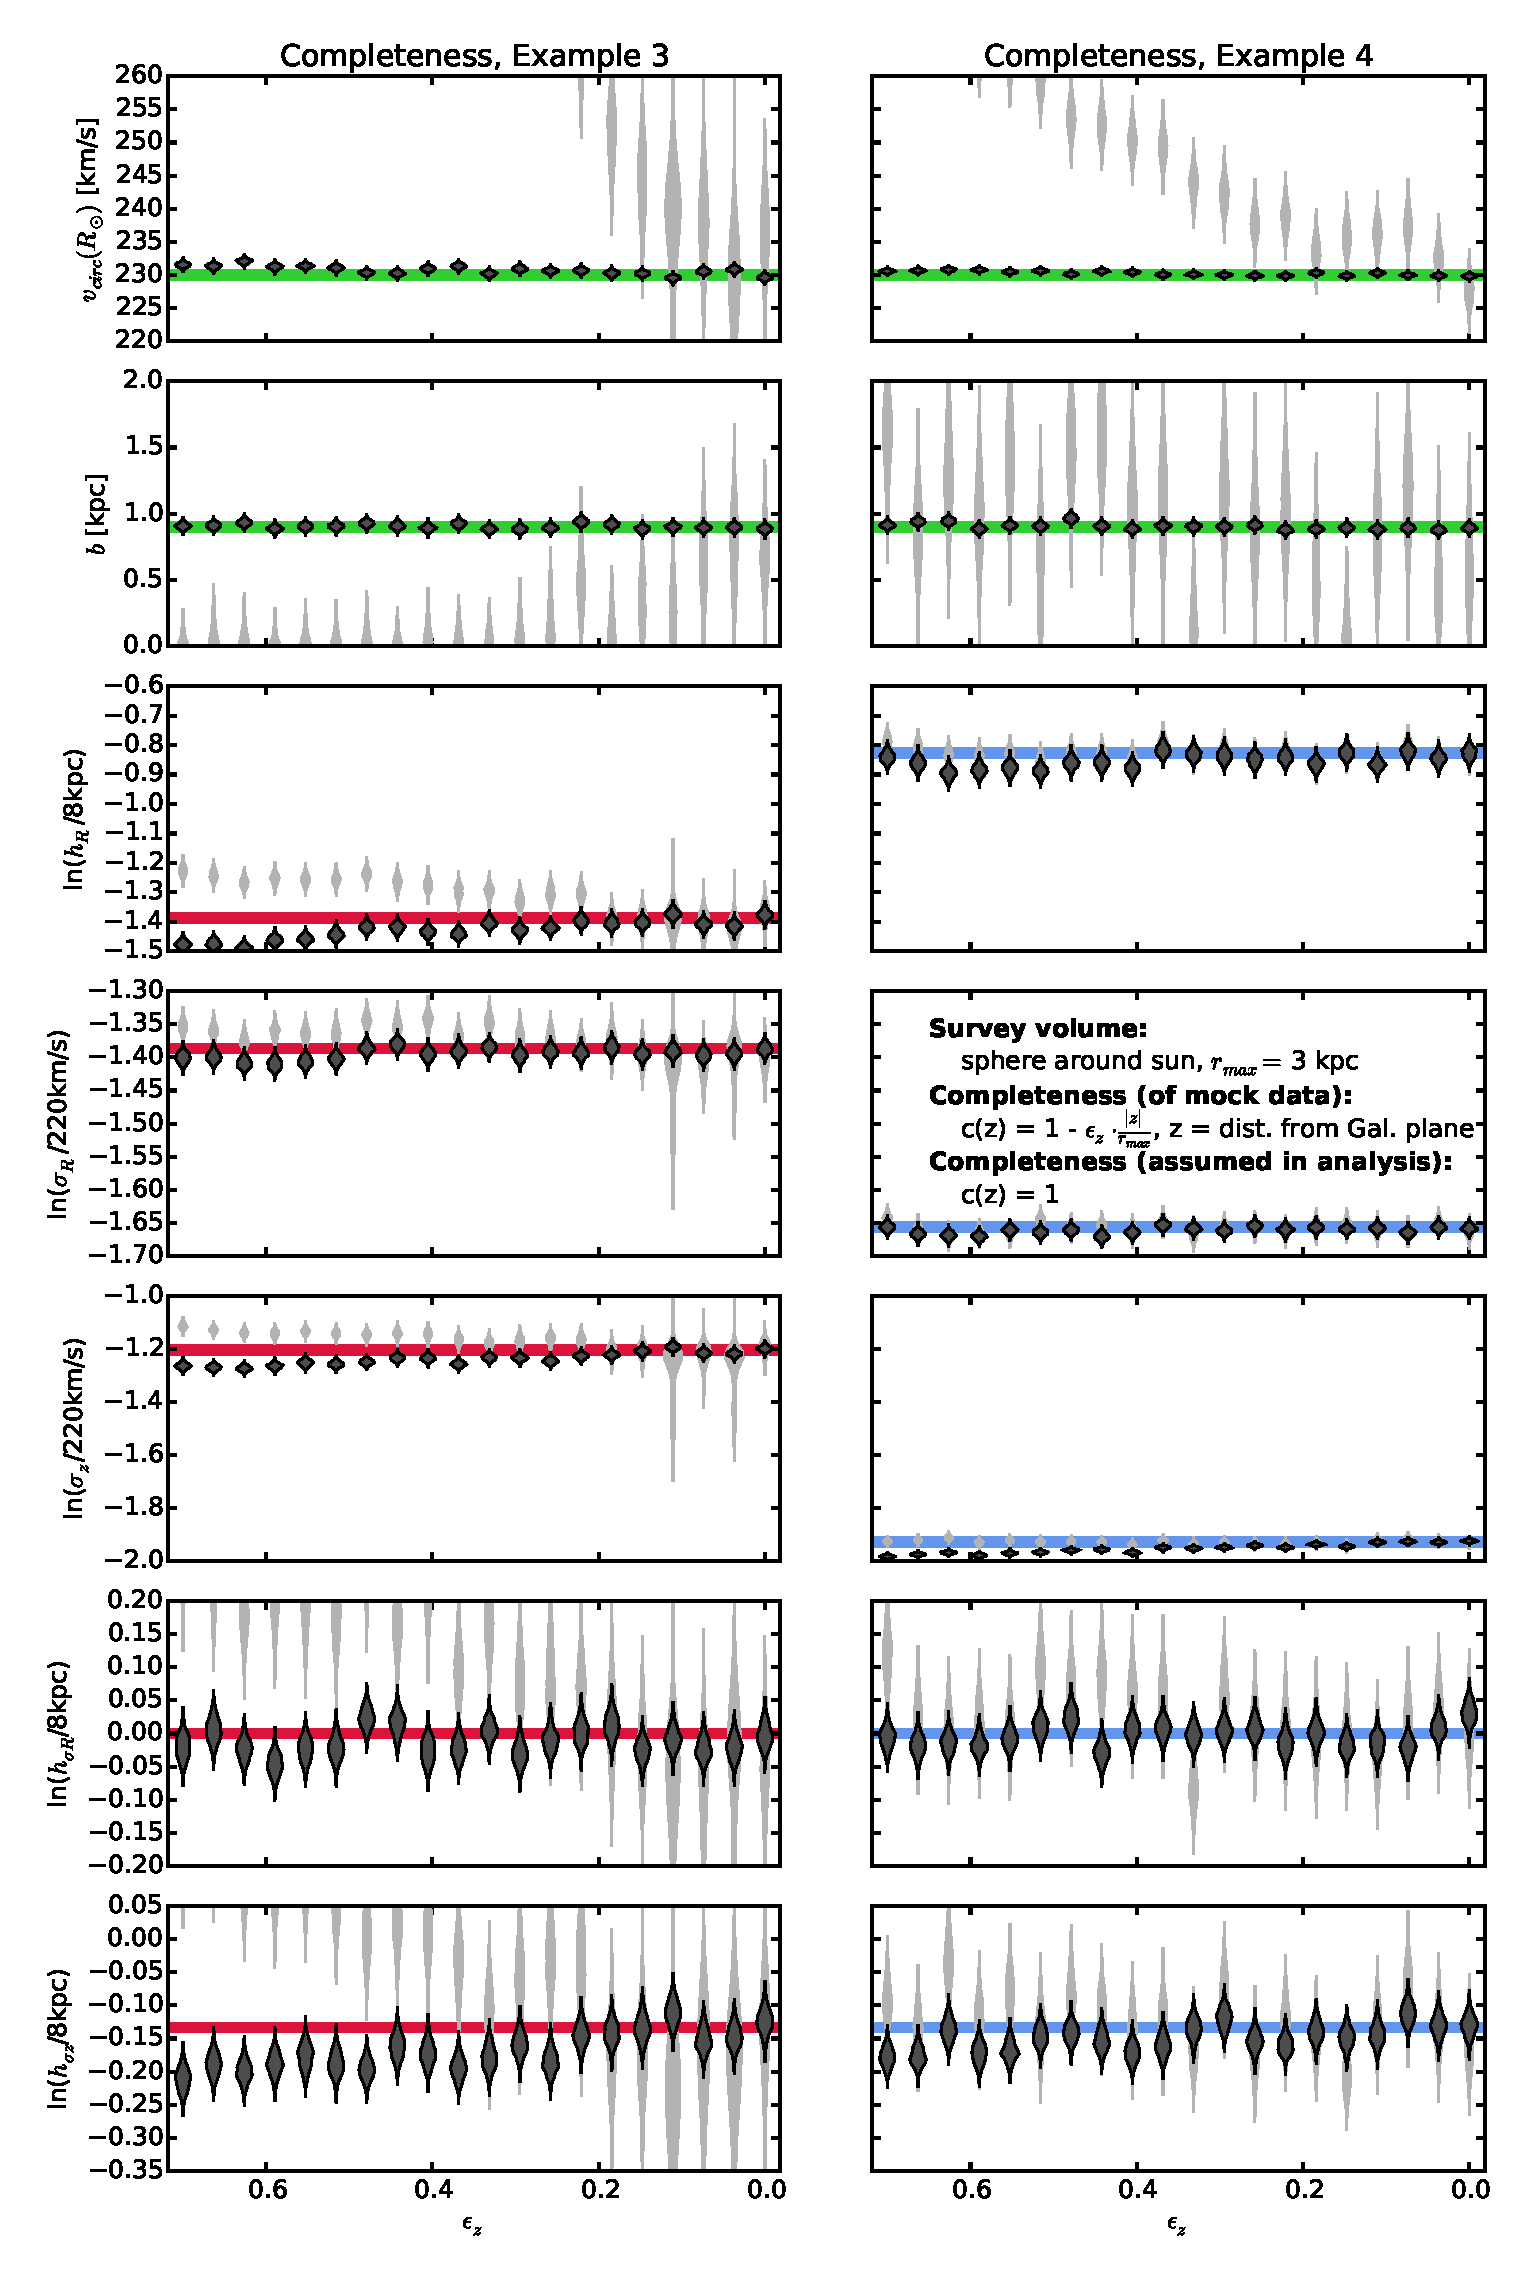
\includegraphics[width=0.8\textwidth]{figs/isoSphFlexIncompZ_violins.eps}
\caption{(Caption on next page.)}
\end{figure*}


\addtocounter{figure}{-1}
\begin{figure*} [t!]
\caption{Influence of wrong assumptions about the incompleteness parallel to the Galactic plane of the data on the parameter reocovery with \RM. Each mock data set was created having different incompleteness parameters $\epsilon_z$ (shown on the $x$-axis and illustrated in Fig. \ref{fig:isoSphFlexIncompZ_mockdata}) and the model parameters are given as test \textcircled{5}, Example 2, in Table \ref{tbl:tests}. The analysis however didn't know about the incompleteness and assumed that all data sets had constant completeness within the survey volume ($\epsilon_z = 0$). The marginalized likelihoods from the fits are shown as violins. The green lines mark the true potential parameters ("Iso-Pot") and the red and blue lines the true qDF parameters ("hot" \MAP in red and "cool" \MAP in blue), which we tried to recover. The \RM method seems to be robust against small to intermediate deviations between the true and the assumed vertical data incompleteness, as well as the radial incompleteness in Fig. \ref{fig:isoSphFlexIncompZ_violins}.} 
\label{fig:isoSphFlexIncompZ_violins}
\end{figure*}

\begin{figure*}
\plotone{figs/isoSphFlexIncomp_marginal_violins.eps}
\caption{Influence of wrong assumptions about radial and vertical incompleteness on the parameter recovery, when \emph{not} including information about the tangential velocities in the analysis. The mock data sets are the same as in Fig. \ref{fig:isoSphFlexIncompR_violins} and \ref{fig:isoSphFlexIncompZ_violins}, but this time we did not include the data coordinates $v_T$ in the analysis and therefore marginalized the likelihood over $v_T$ instead (see \S\ref{sec:incompZ}). This demonstrates that a lot of information about the potential is actually stored in the rotation curve, i.e. $v_T(R)$, which is not affected by removing stars from the data set. But even if we do not include $v_T$ we can still recover the potential within the errors, at least for small ($\epsilon_z \lesssim 10\%$).} 
\label{fig:isoSphFlexIncomp_marginal_violins}
\end{figure*}
}
\end{appendix}

\section{Questions that haven't been covered so far:}

\begin{itemize}
\item What limits the overall code speed?
\item What happens, when the errors are not uniform?
\item What if errors in distance matter for selection?
\item Deviations from axisymmetry: Take numerical simulations.
\end{itemize}

\paragraph{Stuff that needs to be further examined about the robustness against data incompleteness:}
\begin{itemize}
\item[[TO DO]] Maybe instead of decreasing completeness with height above the plane, a completeness
that INcreases with height above the plan, to model e.g. obscuration due to dust.
\item[[TO DO]] Make similar test as isoSphFlexIncompR, but with KKS potential, to test, if this
robustness is a special case for the isochrone potential.
\end{itemize}

\paragraph{General Stuff}
\begin{itemize}
\item[[TO DO:]] Rename everywhere $N_\text{sigma}$ to $n_\text{interval}$ or something like this.
\item[[TO DO:]] Look up what McMillan \& Binney 2013 have to say about the numerical accuracy of the normalisation. Sanders \& Binney (2015) are quoting them on that matter.
\item[[TO DO:]] Consistent capitals in section titles.
\item[[TO DO:]] Make consistent: use of $\sigma_{R,0}$ and $\sigma_R$ as profile or dispersion at sun.
\item[[TO DO:]] Make consistent $h_{\sigma_R}$ --> $h_{\sigma,R}$
\item[[TO DO:]] Make consistent $M$ --> \pmodel
\item[[TO DO:]] Make consistent MAP --> \MAP
\item[[TO DO:]] Make consistent number of stars $N$ --> $N_\text{sample}$, introduce somewhere
\item[[TO DO:]]  introduce \pdf somewhere
\end{itemize}

%=====================================================

%15. May 2015 --> Meet with HW to write
%
%* just explain what the best solution in analysis section is, don't explain too much about other (worse) techniques
%* Numerical accuracy plot is a result
%* 20,000 stars --> much larger than current sample sizes (200 stars), but forecasting to larger sample sizes with Gaia (?)
%* Fig. 3,4,5 --> Behaviour in the limit of large samples
%* Change order of sections according to order in Results section intro
%* mention in introduction that we do not investigate axisymmetry
%* limit of lousy data --> model assumptions are not limiting. very good data --> model assumptions are limiting. Bovy & Rix: 150 stars per MAP. When we get larger samples sizes, the modelling will be limited by the model assumptions.
%* rename model parameters $M$ into $p_M$
%* mock data in action space plot --> in mock data section
%* accuracy plot --> in "Numerical accuracy of the likelihood calculation" section
%* in section on numerical accuracy erwähnen, dass wir in the limit of many stars aufpassen müssen, dass wir die normalisierung genau genug berechnen.
%* Macro fuer MAP schreiben: In Kapitälchen, damit klar ist, dass das ein Akronym ist
%* Citation korrigieren: bo13 --> bov13
%* Check how many stars were typically in a Bovy&Rix13 MAP
%* Triangle plot --> I talk about likelihood, but it is a pdf!
%* Priors: We want parameter estimates that alre tight enough, such that it does not matter, if we had assumed a flat or a logarithmically flat prior
%* Introduce somewhere the 20,000 stars 
%* if the priors are sufficiently flat, likelihood and pdf are the same.
%* rename $N_j$ into $N_sample$
%* change <_ 1 in eq. 5 to <_ 1/N_sample
%* Mach einheitlich: width of pdf, likelihood, Standard error --> $\sigma_p$ ???
%* schwarze punkte in (un)-bias CLT plot: call "pdf expectation value"
%* triangle plot: potential-potential, qdf-qdf und potential-qdf panels in unterschiedlichen Farbschemen.
%* Error on the width of the likelihood scales also with 1/sqrt(N) or sqrt(N-1) --> nicht in sqrtN figure einzeichnen, weil mein scatter größer ist. Neu berechnen?
%* Latex Tipp: ~ ist ein halber Abstand.
%* TO DO: Test, if characteristic errors indeed smaller than disp --> negligible
%* obsvolumetest: orange volume eine breite weiter nach oben, also leicht oberhalb der plane.
%* replace "cf." with "see" everywhere
%* Latex Tipp: Häufige Bennenungen als Befehle definieren. Lässt sich nachträglich leichter ändern.
%* Check that CLT plot and volumetestplot have both 20,000 stars
%* epsilon ist was kleines, sollte also nicht 100% sein (incompleteness ...)

%26. June 2015 --> Meet with HW to write
%* Make consistent: fig. --> Fig., table --> Table, eq. --> Eq.
%* change examples 1-4 to examples 1a/b and 2a/b
%* reference always in text that exact model parameters are mentioned in figure caption
}







%
[TO DO: Check if all references are actually used in paper. ???]

\begin{thebibliography}{}
\bibitem[Batsleer \& Dejonghe(1994)]{bat94} [TO DO]
\bibitem[Binney(2010)]{bin10} Binney, J. J. 2010, MNRAS, 401, 2318
\bibitem[Binney \& McMillan(2011)]{bin11} Binney, J. J., \& McMillan, P. 2011, \mnras, 413, 1889
\bibitem[Binney(2012)]{bin12} Binney, J. J. 2012a, \mnras, 426, 1324
\bibitem[Binney(2012)]{bin12b} Binney, J. J. 2012b, \mnras, 426, 1328 (Princeton University Press)
\bibitem[Binney \& Tremaine(2008)]{bin08} Binney, J., \& Tremaine, S. 2008, [TO DO: Galactic Dynamics???]
\bibitem[Bovy \& Tremaine(2012)]{bt12} Bovy, J., \& Tremaine, S. 2012, \apj, 756, 89
\bibitem[Bovy et al.(2012b)]{bov12b} Bovy, J., Rix, H.-W., \& Hogg, D. W. 2012b, \apj, 751, 131
\bibitem[Bovy et al.(2012c)]{bov12c} Bovy, J., Rix, H.-W., Hogg, D. W. et al., 2012c, \apj, 755,115
\bibitem[Bovy et al.(2012d)]{bov12d} Bovy, J., Rix, H.-W., Liu, C. et al., 2012d, \apj, 753, 148
\bibitem[Bovy \& Rix(2013)]{bov13}  Bovy, J., \& Rix, H.-W. 2013, \apj, 779, 115
\bibitem[Bovy(2015)]{bov15} [TO DO] Bovy (2015) Galpy paper
\bibitem[Dehnen \& Binney(1998)]{deh98} Dehnen, W., \& Binney, J. 1998, \mnras, 294, 429
\bibitem[Gilmore \& Reid(1983)]{gil83} Gilmore, G. \& Reid, N. 1983, \mnras, 202, 1025
\bibitem[McMillan(2011)]{mcm11} McMillan, P. 2011, \mnras, 414, 2446
\bibitem[Ness et al.(2015)]{nes15} Ness, M., Hogg, D. W., Rix, H.-W. et al., 2015 [TO DO????]
\bibitem[Piffl et al.(2014)]{pif14} Piffl, T., Binney, J., \& McMillan, P. J. et al., 2014, \mnras, 455, 3133
\bibitem[Rix \& Bovy(2013)]{rix13} Rix, H.-W., \& Bovy, J. 2013, [TO DO] A\& ARv, 21, 61
\bibitem[Sackett(1997)]{sac97} Sackett, P. 1997, \apj, 483, 103
\bibitem[Sanders \& Binney(2015)]{san15} [TO DO] Sanders \& Binney (2015) Extended distribution functions for our Galaxy
\bibitem[Steinmetz et al.(2006)]{ste06} Steinmetz, M. et al., 2006, \aj, 132, 1645
\bibitem[Ting et al.(2013)]{tin13} Ting, Y.-S., Rix, H.-W., Bovy, J., \& van de Ven, G. 2013, \mnras, 434, 652
\bibitem[Zhang et al.(2013)]{zha13} Zhang, L., Rix, H.-W., van de Ven, G. et al., 2013, \apj, 772, 108
\end{thebibliography}

[TO DO: Mit wie vielen J. wird Binney geschrieben?] [TO DO: Kommas nach letztem Namen oder nicht?] [TO DO: In welcher Reihenfolge soll ich sortieren?] [TO DO: Wie viele Autoren nennen, bevor et al.???]



\end{document}

